\documentclass{article}

\usepackage{Engineering}
\pdftitle{Electrical-eng}

% === TEXT ===
\title{\textbf{Electrical Engineering \\ HSLU, Semester 2}}
\author{Matteo Frongillo}
\date{}

\begin{document}

\maketitle
\tableofcontents
\pagebreak

\part{...}
\section{...}
\subsection{Current strength or current ``I''}
\begin{center}
    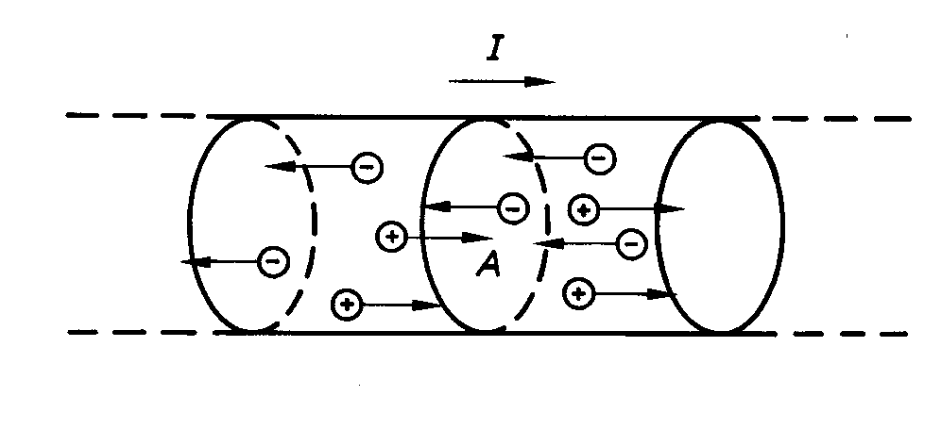
\includegraphics[width=.4\textwidth]{media/intensity.png}
\end{center}
\[I\ [A] =\dfrac{\text{el. charge}}{t}\]

\subsection{Current density ``J''}
\begin{center}
    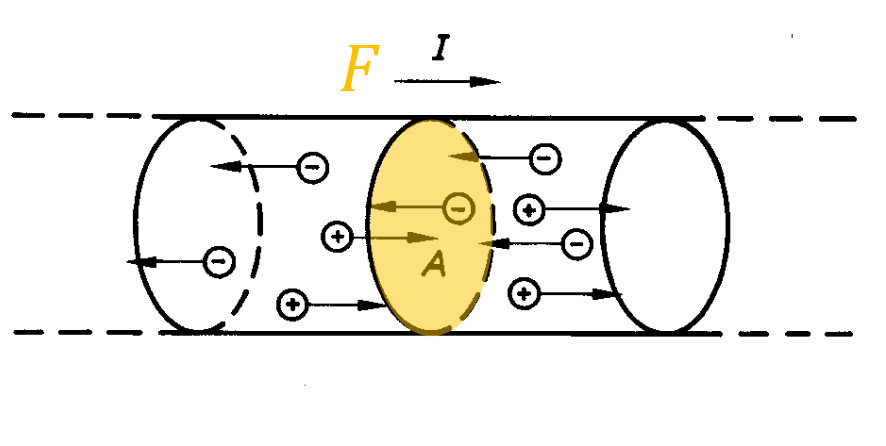
\includegraphics[width=.4\textwidth]{media/density.png}
\end{center}
The current density indicates how large the current per cross-sectional area (F) is:
\[J\ [\dfrac{A}{mm^2}] = \dfrac{I}{F}\]

\subsection{Temperature dependence of the resistance}
\begin{center}
    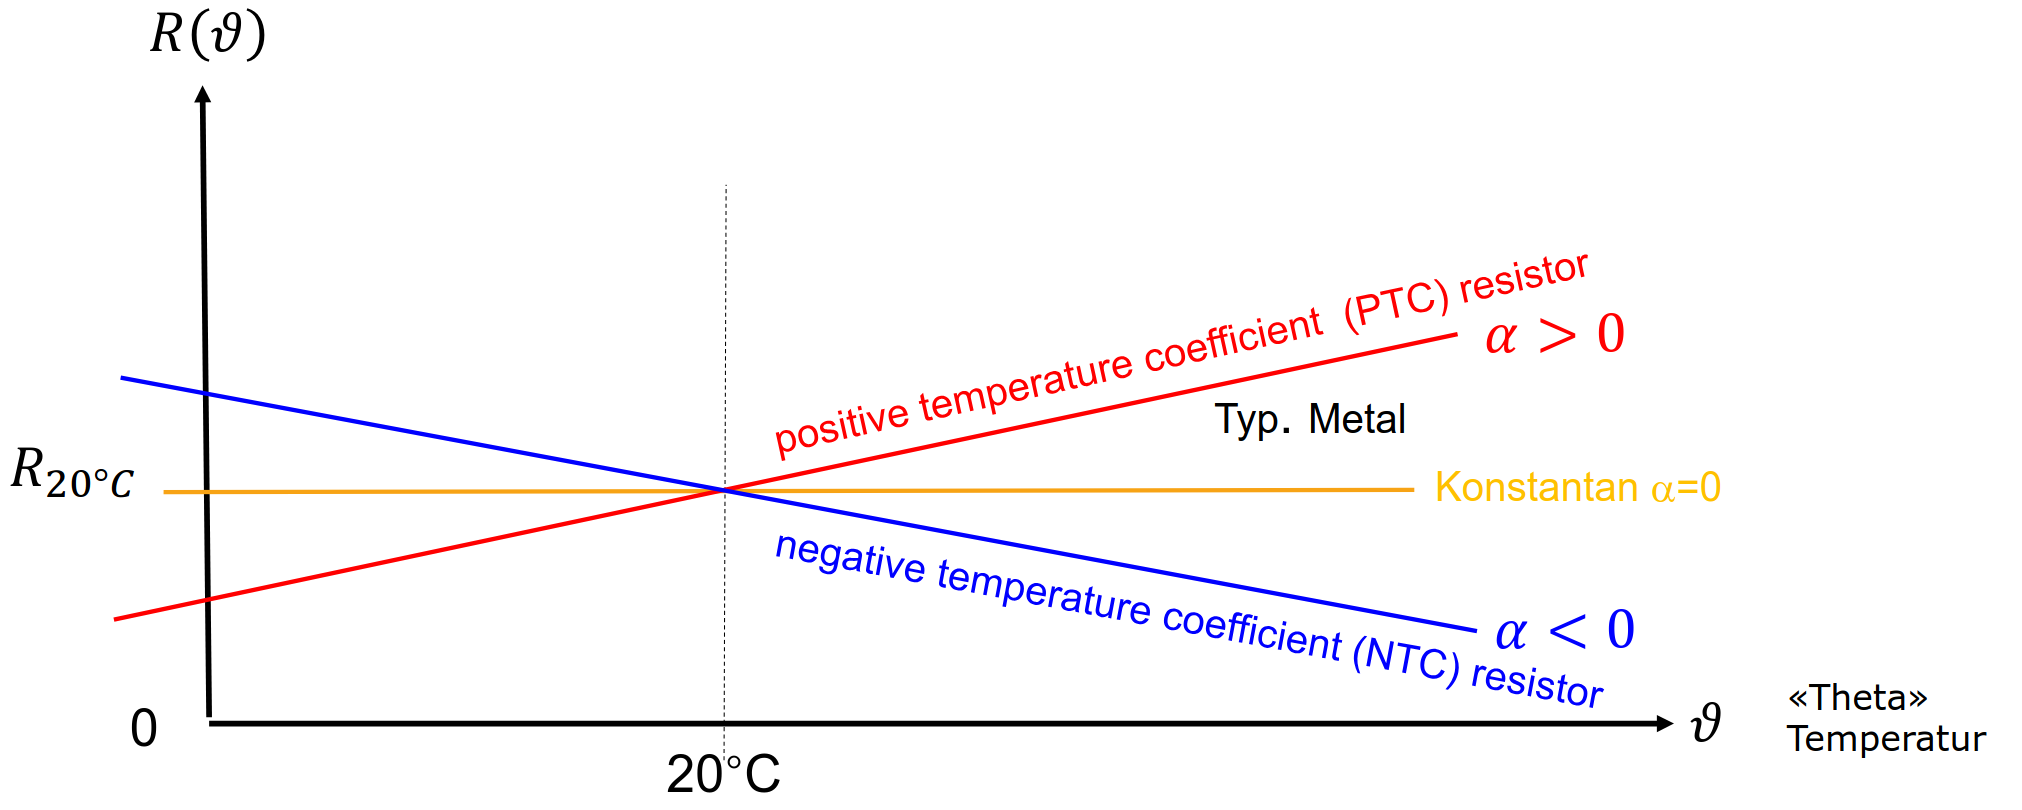
\includegraphics[width=\textwidth]{media/resistance.png}
\end{center}
Depending on the material, the resistance can increase, remain the same or decrease with temperature. In
ET+L we calculate using the linear approach.
\figbox{$R(\vartheta) = R_{20}(1+\alpha(\vartheta-20^{\circ}\text{C})) = R_{20}(1+\alpha \Delta T)$}

\subsection{Object properties}
The resistance indicates the voltage required for a
current. In addition to the material, the cross-sectional
area and also the length are decisive factors.
\[R=\frac{U}{I}\]

\subsection{Reciprocal quantities}
\subsubsection{Specific resistance}
To describe material properties, the resistance per length
and cross-sectional area is specified (precondition:
homogeneous conductor, direct current):
\[\rho\ [\frac{\Omega \cdot mm^2}{m}] = R\cdot \frac{A}{l}\]

\subsubsection{Conductance}


\subsubsection{Specific conductivity}

\newpage
\section{Gravitational fields}
\subsection{Between bodies}
\efigbox{F_1 = F_2 = G\dfrac{m_1m_2}{d^2}}

\subsection{Between particles}
\subsubsection{Coulomb's law}
It calculates the amount of force between two electrically charged
particles at rest:
\efigbox{F=\dfrac{1}{4\pi \varepsilon_0} \cdot \dfrac{q_1q_2}{r^2}}

where:
\begin{itemize}
    \item $F$: Force [N];
    \item $q$: Charge [As];
    \item $\varepsilon_0$: absolute permittivity = $8.8542\cdot 10^{-12}$ [As/Vm].
\end{itemize}

\subsection{Electric field and force on a charge $Q$}
\subsubsection{Homogeneous electric fields}
\efigbox{E=\dfrac{U}{d}}

where:
\begin{itemize}
    \item $E$: electric field strength [V/m];
    \item $U$: voltage [V];
    \item $d$: distance of the electrodes [m].
\end{itemize}

\subsubsection{Force on a point charge}
\efigbox{F=Q\cdot E}

where:
\begin{itemize}
    \item $E$: electric field strength [V/m];
    \item $Q$: charge [As];
    \item $F$: force [N].
\end{itemize}

\newpage
\section{Capacitance and Capacitor}
\subsection{Capacitor}
A capacitor is a device in which the capacitance is used.

\subsection{Capacitance}
Capacitance $C$ is the \textbf{capability} to store electric charge.
It is measured by the charge divided by the applied voltage:
\efigbox{C=\dfrac{Q}{U}}

where:
\begin{itemize}
    \item $Q$: charge [As];
    \item $U$: voltage [V];
    \item $C$: capacitance [As/V = F (Farad)].
\end{itemize}

\subsubsection{Capacitance of a plate capacitor}
\efigbox{C=\varepsilon\cdot \dfrac{A}{d}}

where:
\begin{itemize}
    \item $A$: plate area (one side) [m$^2$];
    \item $d$: distance between plates [m];
    \item $C$: capacitance [F].
\end{itemize}

\pph{Permittivity}
\efigbox{\varepsilon = \varepsilon_r\cdot \varepsilon_0}
\begin{itemize}
    \item $\varepsilon_r$: relative permittivity of the dielectric, relative to the air;
    \item $\varepsilon_0$: absolute permittivity [As/Vm].
\end{itemize}

\subsubsection{Energy in a capacitor}
If a capacitor is discharged with a constant current, the voltage decreases linearly:

\efigbox{\int_{0}^{t_{\text{empty}}}U(t)\cdot I\,dt = I\cdot U_0 = \frac{I\cdot U_0 \cdot t_{\text{empty}}}{2}}

Or, simplified:
\efigbox{W=\frac{1}{2}C\cdot U_0^2}

where:
\begin{itemize}
    \item $W$: energy [J or Ws];
    \item $U_0$: initial voltage [V];
    \item $C$: capacitance [F].
\end{itemize}

\subsection{Capacitors in parallel connection}
Capacitances connected in parallel add up:
\efigbox{C_{\text{tot}} = \frac{\sum_{n} Q_n}{U} = \sum_{n} C_n}

or

\efigbox{C = \frac{\varepsilon\cdot \left(\sum_{n} A_n\right)}{d} = \sum_{n} C_n}

\subsection{Capacitors in series connection}
In a series connection, the reciprocal of the total capacitance is the sum of the reciprocals of the individual capacitances:
\efigbox{\frac{1}{C_{\text{tot}}} = \sum_{n}\frac{1}{C_n}}

where:
\begin{itemize}
    \item $C_{\text{tot}}$: total capacitance [F];
    \item $C_n$: capacitance of the $n$-th capacitor [F].
\end{itemize}

\section{Transient Analysis in RC Circuits}
\subsection{Charging of a Capacitor}
When a capacitor is charged through a resistor, the voltage across it increases exponentially:
\efigbox{U_C(t)= U_0\cdot\left(1-e^{-t/(R\cdot C)}\right)}

with the time constant defined as:
\efigbox{\tau=R\cdot C}

where:
\begin{itemize}
    \item $U_C(t)$: voltage across the capacitor at time $t$ [V];
    \item $U_0$: applied voltage [V];
    \item $R$: resistance [$\Omega$];
    \item $C$: capacitance [F];
    \item $\tau$: time constant [s].
\end{itemize}

\subsection{Discharging of a Capacitor}
When a charged capacitor discharges through a resistor, the voltage decays exponentially:
\efigbox{U_C(t)= U_0\cdot e^{-t/(R\cdot C)}}

and the discharging current is:
\efigbox{I(t)= \frac{U_0}{R}\cdot e^{-t/(R\cdot C)}}

\newpage
\subsection{Transitional phase}
\efigbox{f(t)=A+\Delta\cdot \left(1-e^{t/\tau}\right) = A+(B-A)\cdot (1-e^{1/\tau})}

\section{Additional Topics}
\subsection{Energy Stored in a Capacitor}
The energy stored in a capacitor is given by:
\efigbox{W=\frac{1}{2}C\cdot U_0^2}

where:
\begin{itemize}
    \item $W$: energy [J];
    \item $C$: capacitance [F];
    \item $U_0$: voltage [V].
\end{itemize}

\subsection{Charge--Voltage Relationship}
For an ideal capacitor, the relationship between charge and voltage is:
\efigbox{Q=C\cdot U}

Moreover, the current is the time derivative of the charge:
\efigbox{I=\frac{dQ}{dt}=C\cdot\frac{dU}{dt}}

Note that the voltage across an ideal capacitor cannot change instantaneously.

\newpage
\section{Electromagnetic fields}
\subsection{Hans Christian Ørsted Observation}
\begin{center}
    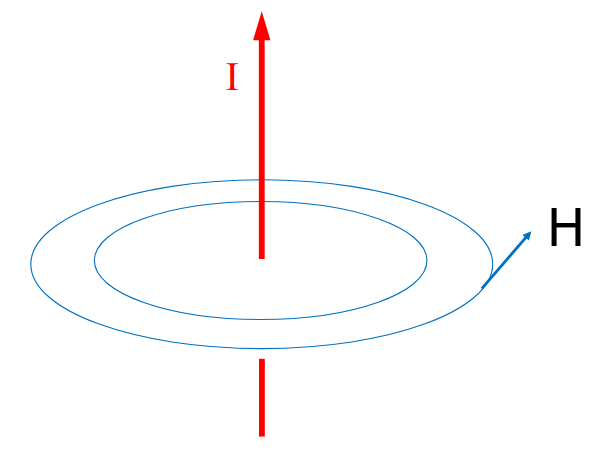
\includegraphics[width=.4\textwidth]{media/observations.png}
\end{center}
\begin{enumerate}
    \item The magnetic field lines encircle the current-carrying conductor;
    \item The magnetic field lines lie in a plane perpendicular to the current-carrying wire;
    \item If the direction of the current is reversed, the direction of the magnetic field lines is also reversed;
    \item The strength of the field is directly proportional to the magnitude of the current;
    \item The strength of the field at any point is inversely proportional to the distance of the point from the wire.
\end{enumerate}

\subsection{Definitions and formuals}
\subsubsection{Magnetomotive force}
\efigbox{\theta = N\cdot I}

\subsubsection{Ampère's circuital law}
\efigbox{\theta = \oint \overrightarrow{H(s)}\cdot \mathrm{d}\vec{s}}

\subsubsection{Magnetic field in a coil}
\begin{center}
    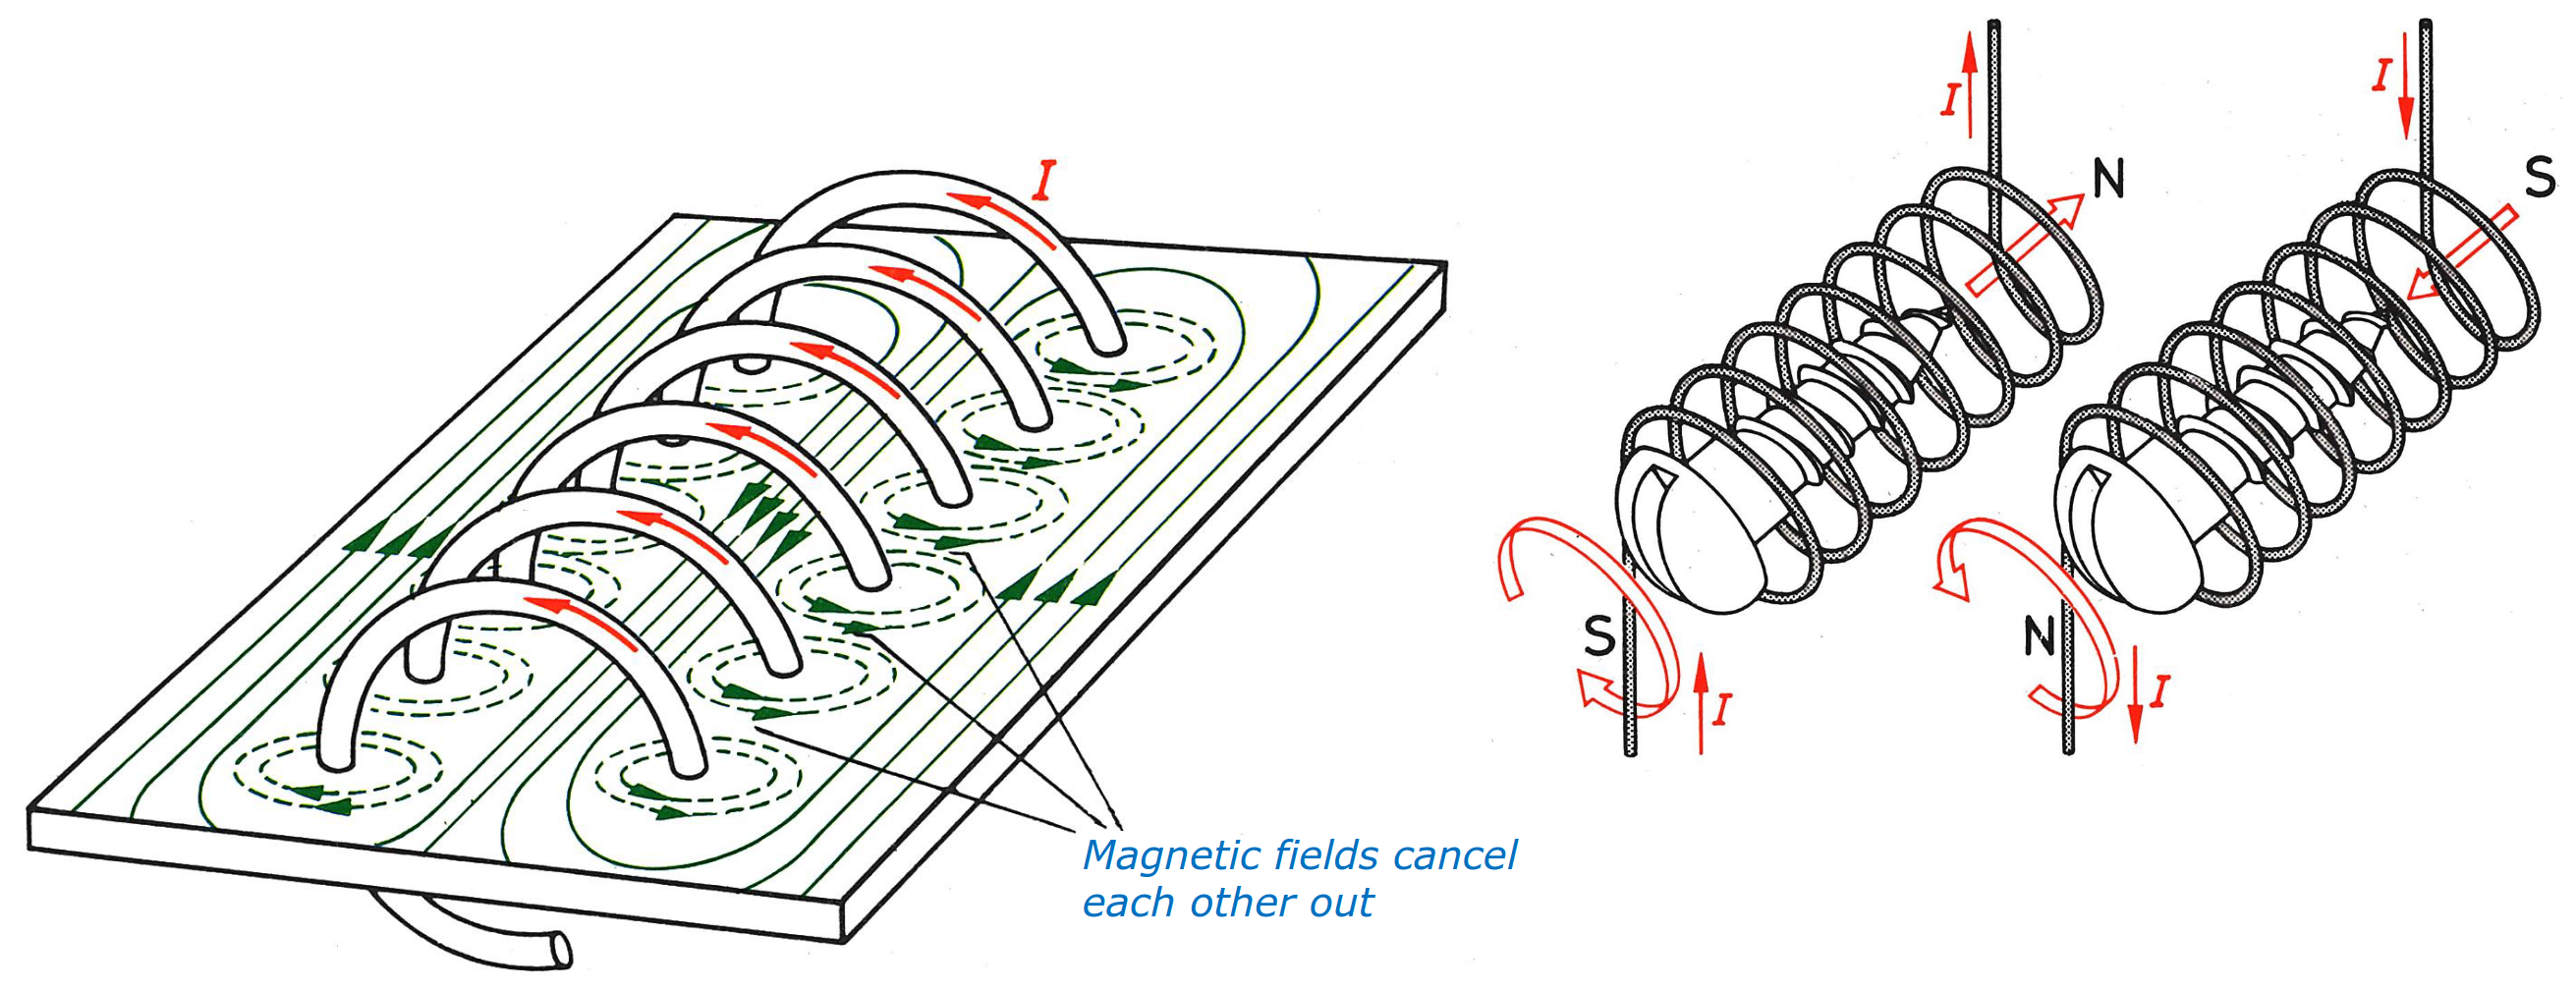
\includegraphics[width=\textwidth]{media/magneticfield_coil.png}
\end{center}

\newpage
\subsubsection{Magnetic flux density}
\efigbox{B = \frac{\Phi}{A} = \mu \cdot H = \mu_0\mu_r\cdot H}

where:
\begin{itemize}
    \item $B$: magnetic flux density [T = Vs/m$^2$];
    \item $\Phi$: magnetic flux [Wb];
    \item $A$: area [m$^2$];
    \item $\mu$: magnetic permeability [H/m = Vs/Am];
    \item $H$: magnetic field strength [A/m];
    \item $\mu_0$: magnetic constant [$4\pi\cdot 10^{-7}$ Vs/Am];
    \item $\mu_r$: relative permeability.
\end{itemize}

\note{$\Phi$ is the sum of all B-field lines through the cross section A}

\subsubsection{Magnetic field strength in coil with iron core}

\begin{center}
    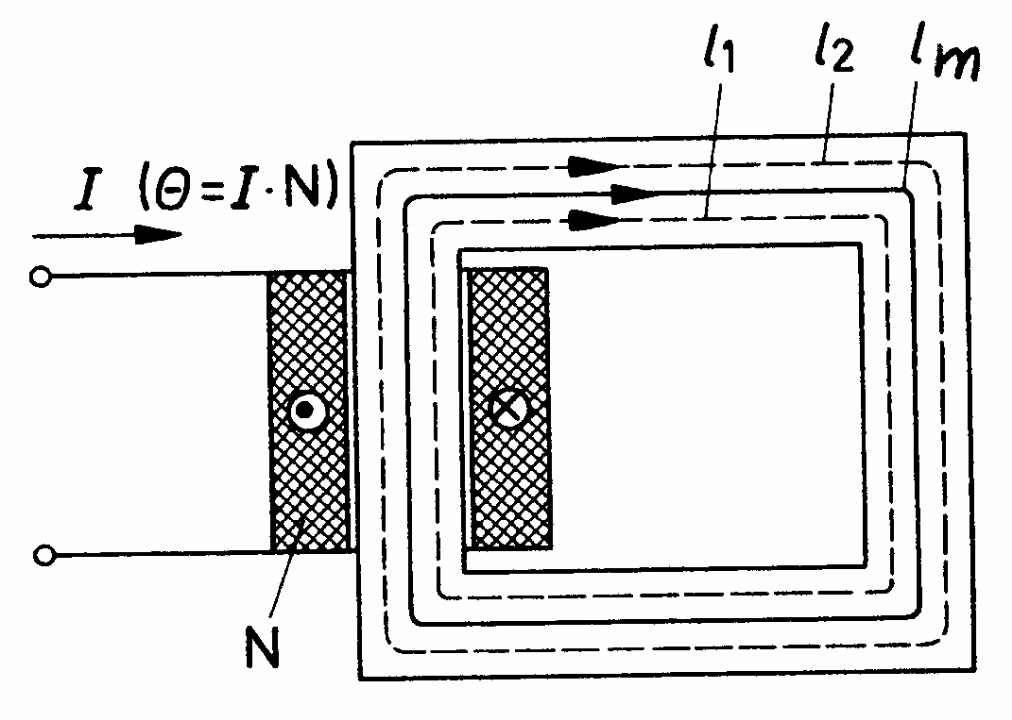
\includegraphics[width=.4\textwidth]{media/strength_iron_core.png}
\end{center}

\efigbox{H = \frac{N\cdot I}{l_{m}} = \frac{\Theta}{l_{m}}}

where:
\begin{itemize}
    \item $H$: magnetic field strength [A/m];
    \item $N$: number of turns;
    \item $I$: current [A];
    \item $l_{m}$: median field line length [m];
    \item $\Theta$: magnetomotive force [A].
\end{itemize}

\subsubsection{Magnetic relative permeability $\mu$}
Permeability is a measure for the ability to conduct magnetic field lines:

\begin{center}
    \begin{tabular}{|l|l|}
        \hline
        \textbf{Material} & $\mathbf{\mu_r}$ \\
        \hline
        Air & 1 \\
        Pure iron & up to 250'000 \\
        Electrical steel & 500 \ldots 7000 \\
        Steel & 40 \ldots 7000 \\
        Water & 0.99991 \\
        \hline
    \end{tabular}
\end{center}

\newpage
\subsubsection{Coils with and without iron core}
The magnetization curve of a coil without a core
is linear, but there is significantly less flux
density B than with an iron core.
\begin{center}
    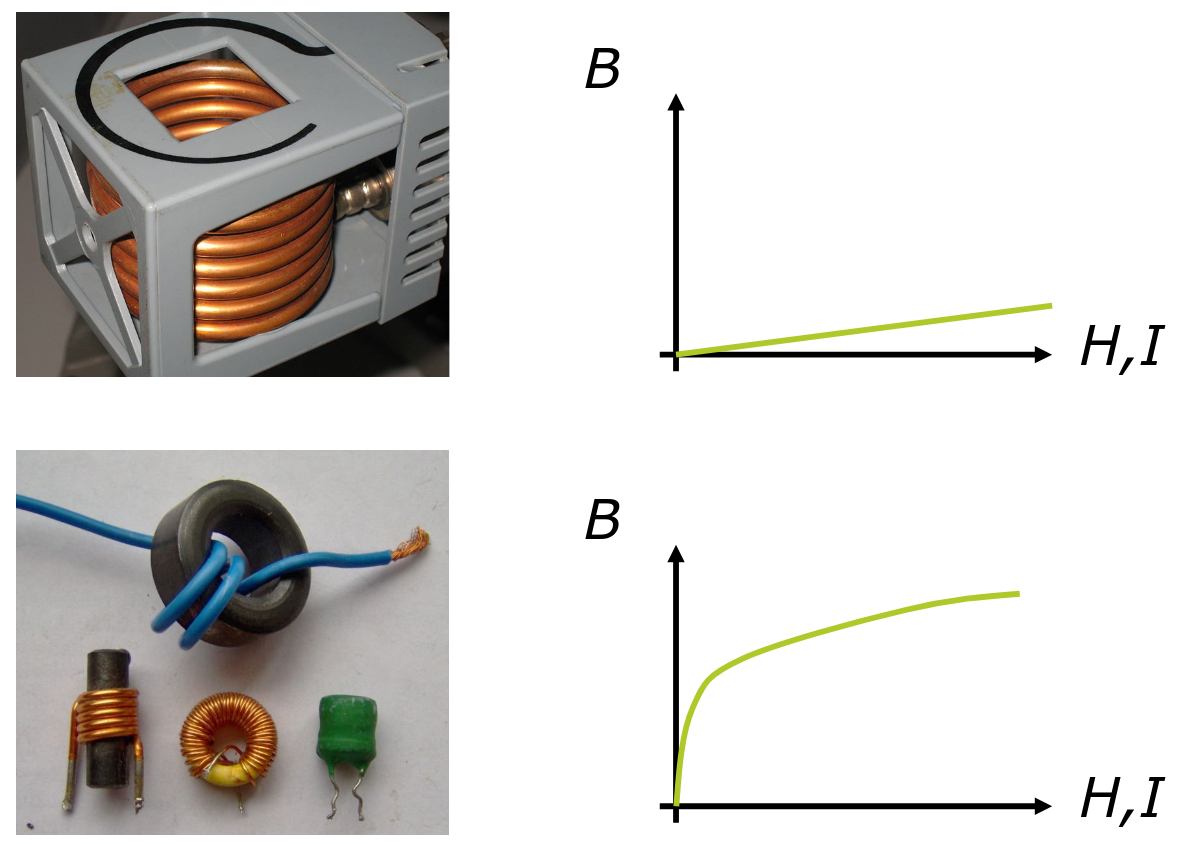
\includegraphics[width=.7\textwidth]{media/iron_coils.png}
\end{center}

\subsubsection{Law of induction and inductance}
\pph{Changing magnetic flux generates a voltage}
\begin{center}
    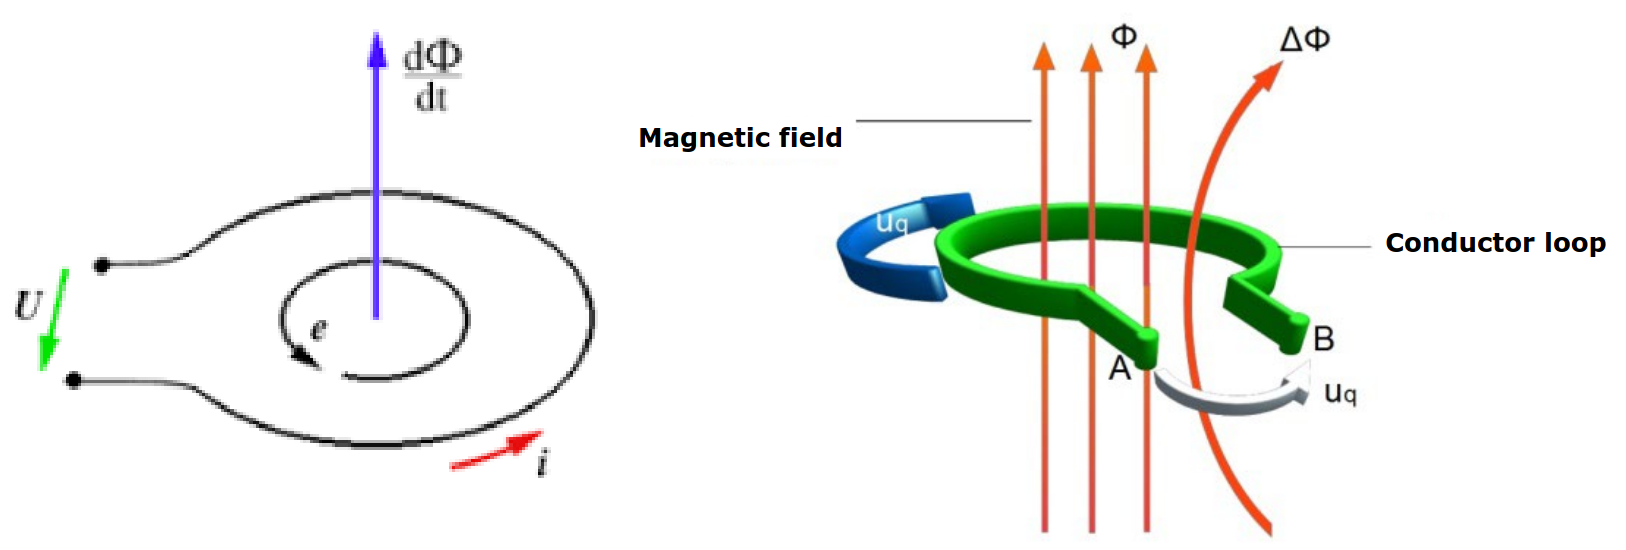
\includegraphics[width=.8\textwidth]{media/law_of_induction.png}
\end{center}

Phenomenon: a changing magnetic flux $\Phi$ induces a
voltage in a conductor loop around it:
\efigbox{U = -N\cdot \frac{\mathrm{d}\Phi}{\mathrm{d}t}}

\newpage
\subsubsection{Inductance and induction}
Inductance L is the capability to generate a magnetic field. It is measured by
the voltage divided by the rate of change of current over time. It is a measure of
the magnetic ``capacity'' of an arrangement of conductors (e.g. coil) and can be
compared to the capacity C of a capacitor. It indicates how much magnetic flux
per ampere is generated.

\efigbox{L = \frac{N\cdot \Phi}{I} = \frac{U}{\frac{\Delta I}{\Delta t}}}

where:
\begin{itemize}
    \item $L$: inductance [H = Vs/A];
    \item $N$: number of turns;
    \item $\Phi$: magnetic flux [Wb];
    \item $I$: current [A];
    \item $U$: voltage [V].
\end{itemize}

\subsubsection{Inductivity of a very long coil}
The inductance of a very long coil can be calculated approximately with:
\efigbox{L = \frac{\mu\cdot N^2\cdot A}{l}}

where:
\begin{itemize}
    \item $L$: inductance [H = Vs/A];
    \item $\mu$: magnetic permeability [Vs/Am];
    \item $N$: number of turns;
    \item $A$: cross-section of the coil [m$^2$];
    \item $l$: length [m].
\end{itemize}

\subsubsection{Energy stored in an inductor}
Since a variable magnetic field induces a voltage in which a current can also flow, the magnetic field must contain
energy:

\efigbox{W = \frac{1}{2}L\cdot I^2}

where:
\begin{itemize}
    \item $W$: work, energy [J = Ws];
    \item $L$: inductance [H = Vs/A];
    \item $I$: current [A].
\end{itemize}

\newpage
\subsubsection{Current-voltage relationship of an inductor}
The current-voltage relationship of an inductor is:
\efigbox{U = L\cdot \frac{\mathrm{d}I}{\mathrm{d}t}}

Special case:
\efigbox{0 = L\cdot \frac{\mathrm{d}I}{\mathrm{d}t} \rightarrow u_c = 0}

\subsubsection{Transient analysis}
\begin{center}
    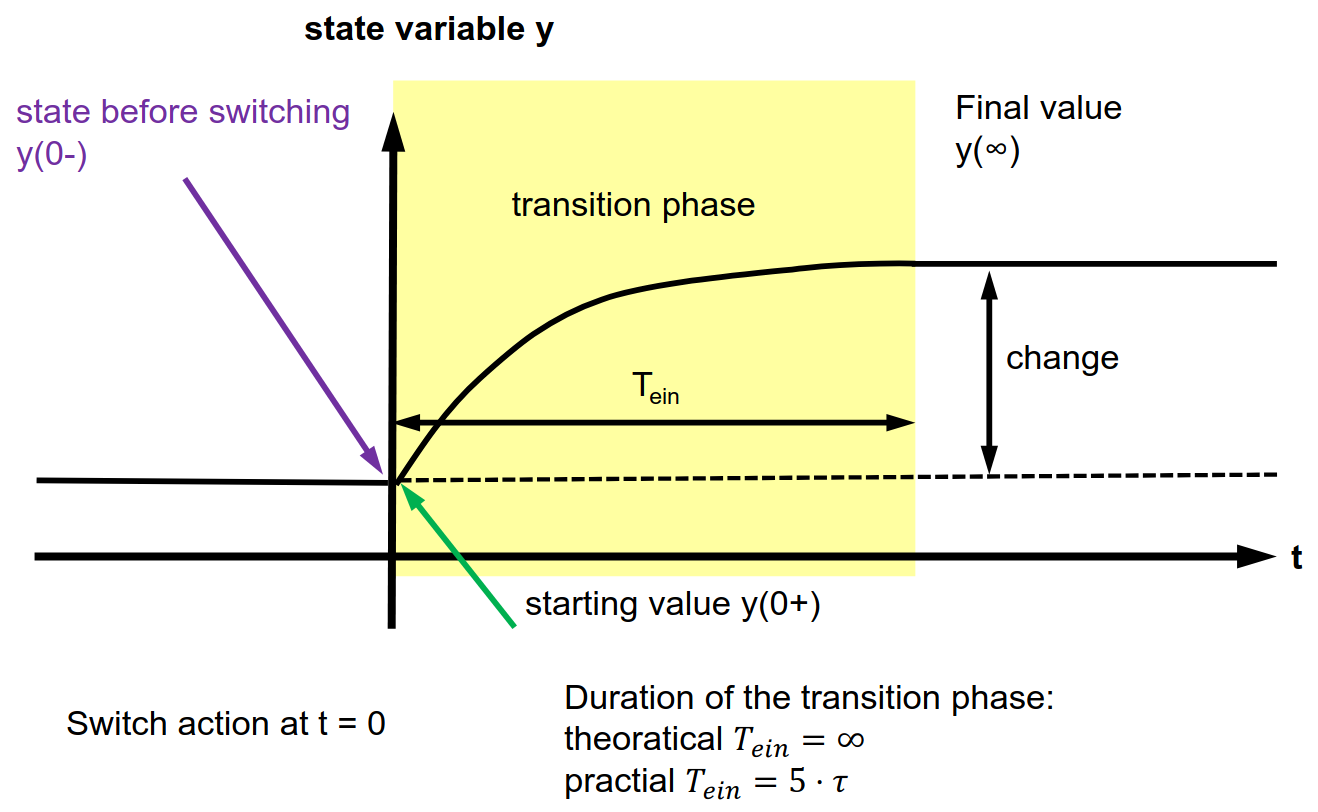
\includegraphics[width=.8\textwidth]{media/transient_analysis.png}
\end{center}

\begin{enumerate}
    \item The state variable $ y(t) $ is the variable that cannot change instantaneously.
    For the inductor, this is $ i_L(t) $. The state just before the switch action:
    \[
      y(0^-) = i_L(0^-).
    \]
  
    \item The starting value is the state immediately before the switch action:
    \[
      y(0^+) = i_L(0) = i_L(0^-).
    \]
    That is, the state variable $ i_L $ keeps the value from $ t = 0^- $.
  
    \item The final value is the value long after the switch action:
    \[
      y(\infty) = i_L(\infty),
    \]
    which is practically reached after $ 5\tau $.
  
    \item The transient is described by the function of time:
    \[
      y(t) = \text{final value}
      + \bigl(\text{starting value} - \text{final value}\bigr)\, \exp{\left(-\frac{t}{\tau}\right)}.
    \]
    Hence,
    \[
      i_L(t) = i_L(\infty)
      + \Bigl(i_L(0+) - i_L(\infty)\Bigr)\, \exp{\left(-\frac{t}{\tau}\right)}.
    \]
\end{enumerate}

\newpage
\pph{Time constant $\tau$ for an inductor}
\efigbox{\tau = \frac{L}{R}}

where:
\begin{itemize}
    \item $\tau$: time constant [s];
    \item $L$: inductance [H];
    \item $R$: resistance [$\Omega$].
\end{itemize}

\subsection{Examples}
\subsubsection{Charging an inductor in a RL-network}
\begin{center}
    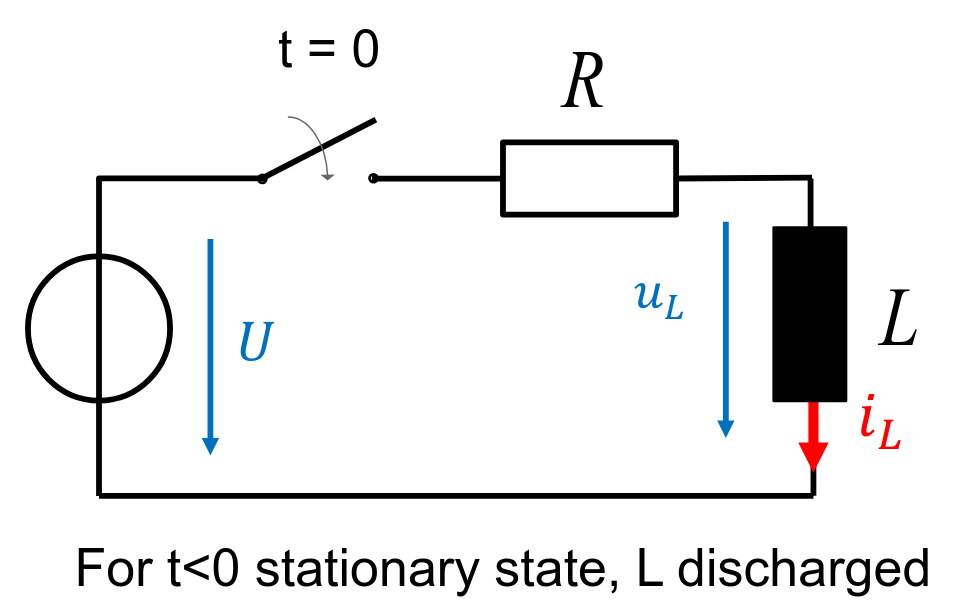
\includegraphics[width=.5\textwidth]{media/inductor_ex1.png}
\end{center}

\pph{Calculations}
\efigbox{i_L = \frac{U}{R}\cdot \left(1-\exp{\left(-\frac{t}{\tau}\right)}\right)\\\\\\
        u_L = U\cdot \exp{\left(-\frac{t}{\tau}\right)}}

\pph{Graphical representation}
\begin{center}
    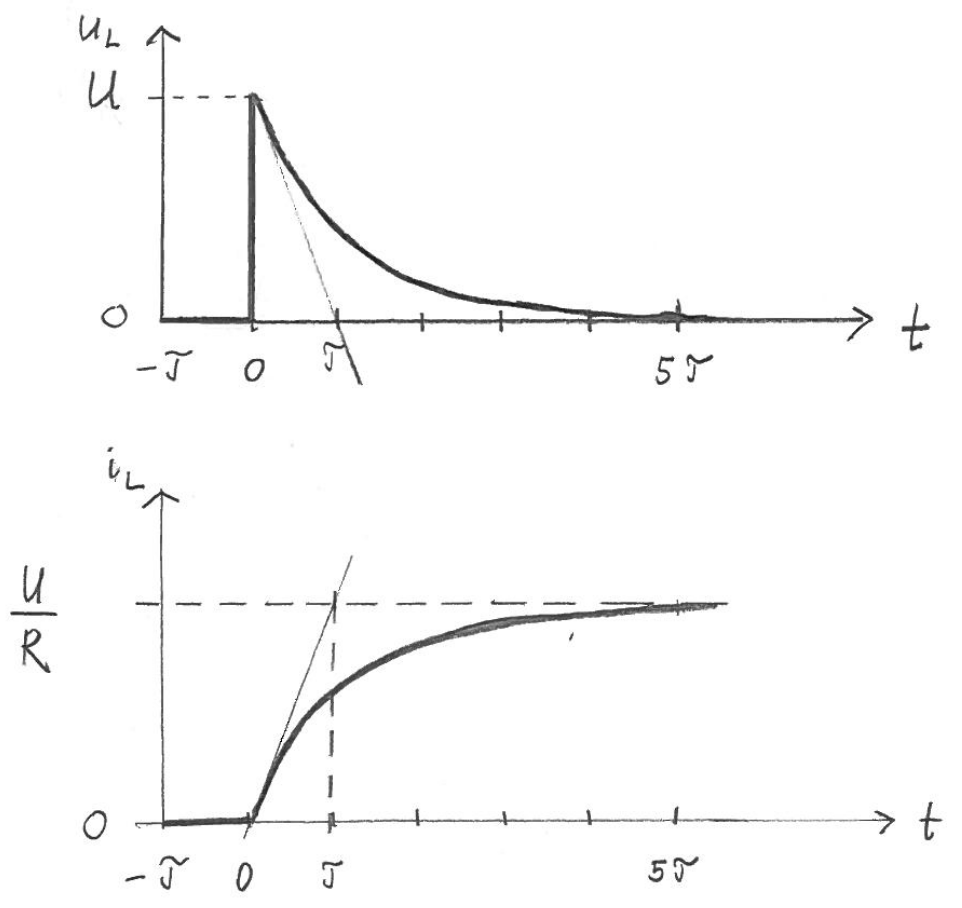
\includegraphics[width=.45\textwidth]{media/inductor_ex1_graph.png}
\end{center}

\newpage
\subsubsection{Discharging an inductor in a RL-network}
\begin{center}
    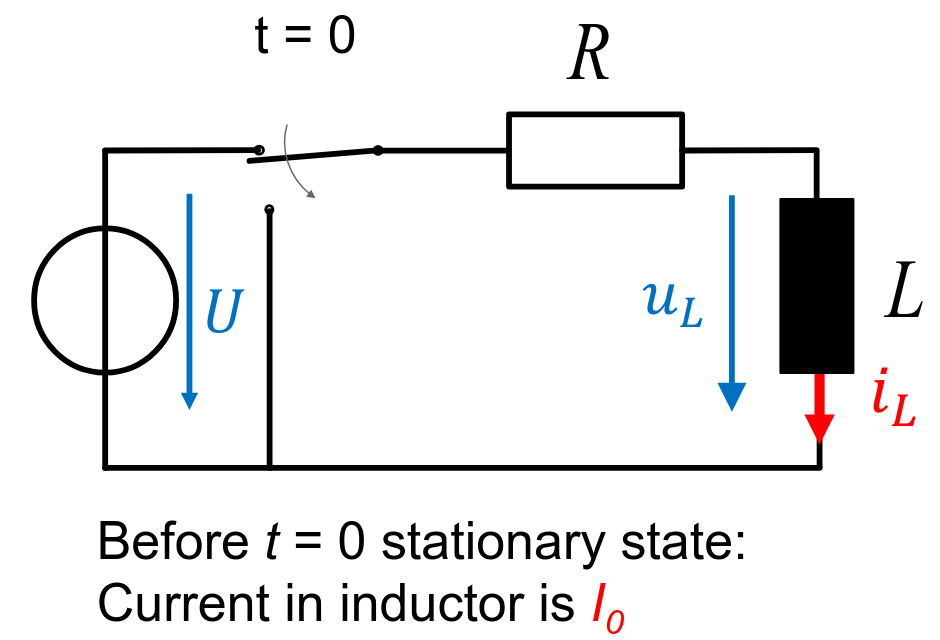
\includegraphics[width=.5\textwidth]{media/inductor_ex2.png}
\end{center}

\pph{Calculations}
\efigbox{i_L = I_0\cdot \exp{\left(-\frac{t}{\tau}\right)}\\\\\\
        u_L = -I_0\cdot R\cdot \exp{\left(-\frac{t}{\tau}\right)}}

\pph{Graphical representation}
\begin{center}
    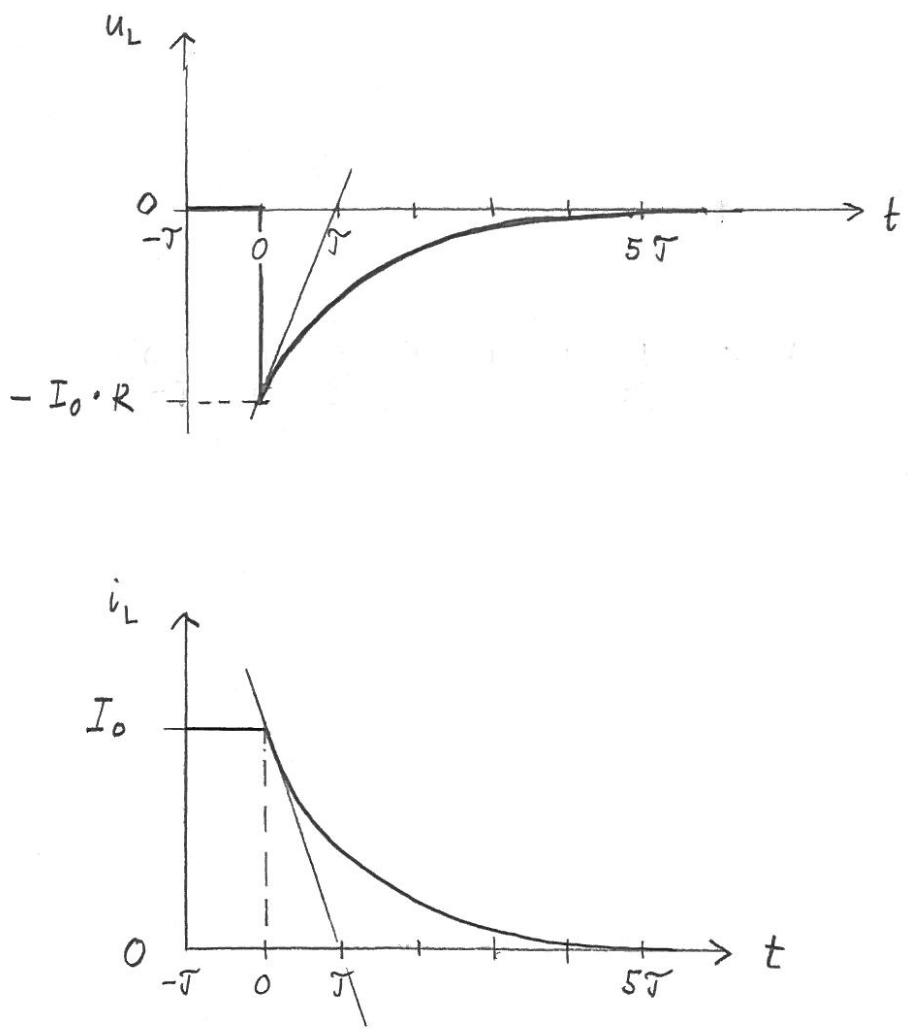
\includegraphics[width=.45\textwidth]{media/inductor_ex2_graph.png}
\end{center}

\newpage
\section{Alternating current (AC)}
\subsection{Generation of alternating current / voltage}
\efigbox{U = -N\cdot \dfrac{\Delta \Phi}{\Delta t}}

where:
\begin{itemize}
    \item $U$: voltage [V];
    \item $N$: number of turns;
    \item $\Phi$: magnetic flux [Wb].
\end{itemize}

\subsection{Comparison of AC and DC}
\begin{figure}[htbp]
    \centering
    % DC Voltage: constant line
    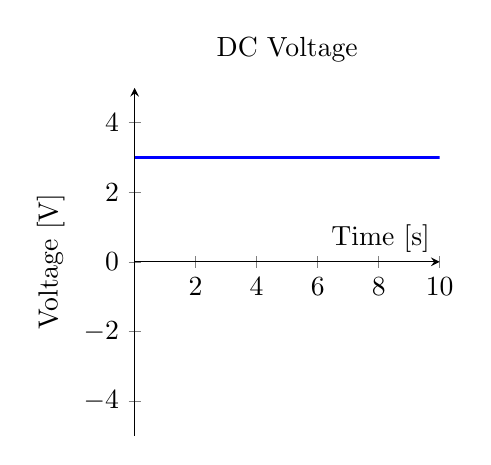
\begin{tikzpicture}
        \begin{axis}[
            width=0.45\textwidth,
            height=6cm,
            xlabel={Time [s]},
            ylabel={Voltage [V]},
            xmin=0, xmax=10,
            ymin=-5, ymax=5,
            title={DC Voltage},
            axis x line=center,
            axis y line=left
        ]
            \addplot [blue, thick, domain=0:10] {3};
        \end{axis}
    \end{tikzpicture}
    \hspace{1cm}
    % AC Voltage: sinusoidal function
    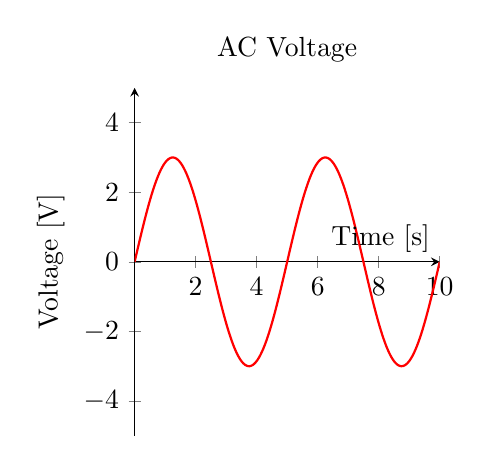
\begin{tikzpicture}
        \begin{axis}[
            width=0.45\textwidth,
            height=6cm,
            xlabel={Time [s]},
            ylabel={Voltage [V]},
            xmin=0, xmax=10,
            ymin=-5, ymax=5,
            title={AC Voltage},
            axis x line=center,
            axis y line=left
        ]
            \addplot [red, thick, samples=200, domain=0:10] {3*sin(deg(2*pi*x/5))};
        \end{axis}
    \end{tikzpicture}
\end{figure}

\begin{minipage}
    {0.5\textwidth}
    \begin{center}
        \begin{flushleft}
            \subsubsection{Advantages of AC}
        \end{flushleft}
        \begin{itemize}
            \item Simple voltage transformation;
            \item Efficient trransmission;
            \item Easier generation;
            \item Compatibility with electric motors.
        \end{itemize}
    \end{center}
\end{minipage}
\begin{minipage}
    {0.5\textwidth}
    \begin{center}
        \begin{flushleft}
            \subsubsection{Disadvantages of AC}
        \end{flushleft}
        \begin{itemize}
            \item Complexity in storage;
            \item Higher risk of shock;
            \item Complex circuits;
            \item Higher rectification costs.
        \end{itemize}
    \end{center}
\end{minipage}

\subsection{Phasors}
\begin{center}
    \begin{tikzpicture}[>=stealth,scale=1.2]
    
        \coordinate (O) at (0,0);
        \coordinate (Z) at (3,2);
        
        \draw[->] (-0.5,0) -- (4.2,0) node[right] {$\mathrm{Re}\,(x)$};
        \draw[->] (0,-0.5) -- (0,3.2) node[right] {$\mathrm{Im}\,(y)$};
        
        \draw[dotted] (Z) -- (3,0);
        \draw[dotted] (Z) -- (0,2);
      
        \fill (Z) circle(1.5pt);
        \node[above right] at (Z) {$z = x + yi$};
      
        \draw[->,thick,blue] (O) -- (Z);
      
        \draw[->,thick,orange]
          (O) -- ++(3*0.95,2*0.95)
          node[midway,above,sloped] {$r$};
      
        \node[below left] at (O) {$O$};
      
        \begin{scope}
          \def\rArc{0.8}
          \draw[red,->] (\rArc,0) arc (0:{atan2(2,3)}:\rArc);
        \end{scope}
        \node[red, below left] at (0.75,0.35) {$\varphi$};
    \end{tikzpicture}
\end{center}

\efigbox{z = x + yi = r\angle \varphi}

\newpage
\subsection{Oscillation as a function of the angle}
Sinusoidal voltage has an instantaneous value $u(t)$ or $u$ for every
time $t$.

After a period of time $T$, the curve repeats itself.

\efigbox{u(t) = \widehat{U} \sin(\omega \cdot t)}

\subsection{Zero phase angle $\varphi$}
\efigbox{u(t) = \widehat{U} \sin(\omega \cdot t + \varphi_u)}

\subsubsection{Phase shift $\Delta\varphi$ between two signals}
\efigbox{u(t) = \widehat{U} \sin(\omega \cdot t + \varphi_u)\\\\
        i(t) = \widehat{I} \sin(\omega \cdot t + \varphi_i)}

The phase shift between two signals is the difference between the
their zero phase signals:
\efigbox{\Delta\varphi = \varphi_u - \varphi_i}

\begin{center}
    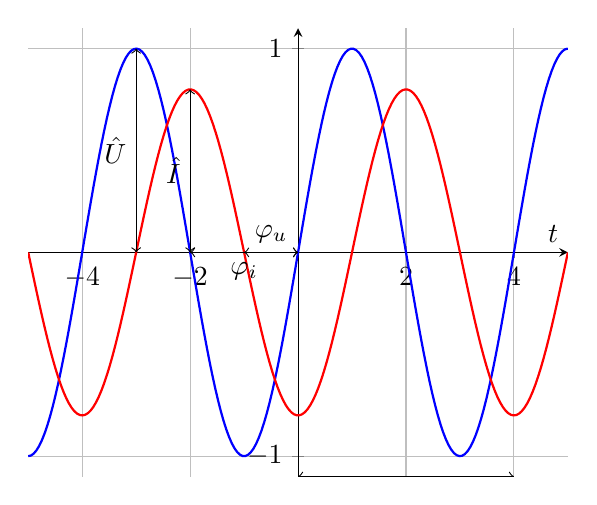
\begin{tikzpicture}
        \begin{axis}[
          axis lines=middle,
          xlabel={$t$},
          xmin=-5, xmax=5,
          ymin=-1.1, ymax=1.1,
          xtick={-4,-2,0,2,4},
          ytick={-1,0,1},
          grid=both
        ]
            \addplot[blue,thick,samples=200] {cos(deg(pi/2*(x+3)))};
            \addplot[red,thick,samples=200] {0.8*cos(deg(pi/2*(x+2)))};
            \draw[<->] (-3,0)--(-3,1) node[midway,left] {$\hat U$};
            \draw[<->] (-2,0)--(-2,0.8) node[midway,left] {$\hat I$};
            \draw[<->] (0,-1.1)--(4,-1.1) node[midway,below] {$T$};
            \draw[<->] (0,0)--(-1,0) node[midway,above] {$\varphi_u$};
            \draw[<->] (0,0)--(-2,0) node[midway,below] {$\varphi_i$};
        \end{axis}
    \end{tikzpicture}
\end{center}

\subsection{Power in a sinusoidal signal and effective value}
\subsubsection{Instantaneous power}
The instantaneous power $p(t)$ is the actual power at a specific time
$t$ and is the product of the voltage $u(t)$ and the current $i(t)$
at that moment:

\efigbox{p(t) = u(t) \cdot i(t) = \dfrac{u(t)^2}{R} = i(t)^2\cdot R}

The active power $P$ corresponds to the mean value of the instantaneous
powerr $p(t)$ averaged over a period $T$:
\efigbox{P = \dfrac{1}{T}\integral[0][T][p(t)][t]}

\newpage
\subsubsection{Effective value}
The effective value $U_{\text{eff}}$ of a sinusoidal signal is the
voltage that would generate the same power in a resistor as the
sinusoidal signal:
\efigbox{U_{\text{eff}} = \sqrt{\dfrac{1}{T}\integral[0][T][u(t)^2][t]} = \dfrac{\widehat{U}}{\sqrt{2}}}

The same can be applied to the effective value $I_{\text{eff}}$:
\efigbox{I_{\text{eff}} = \dfrac{\widehat{I}}{\sqrt{2}}}

\subsection{Relationship between current and voltage on a capacitor}
\begin{center}
    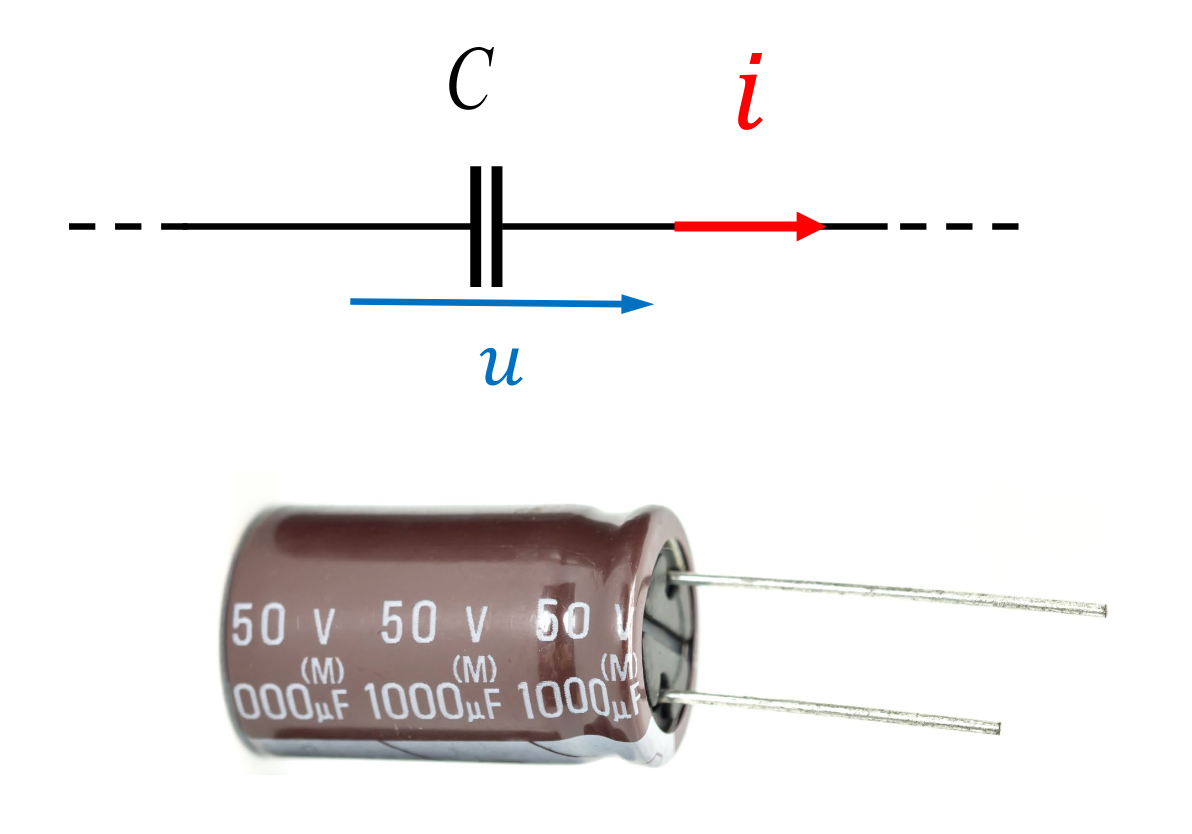
\includegraphics[width=.3\textwidth]{media/capacitor_i_u.png}
\end{center}

\efigbox{i = C\cdot \dfrac{\Delta u}{\Delta t}}

\subsection{Capacitive reactance $X_c$}
\begin{center}
    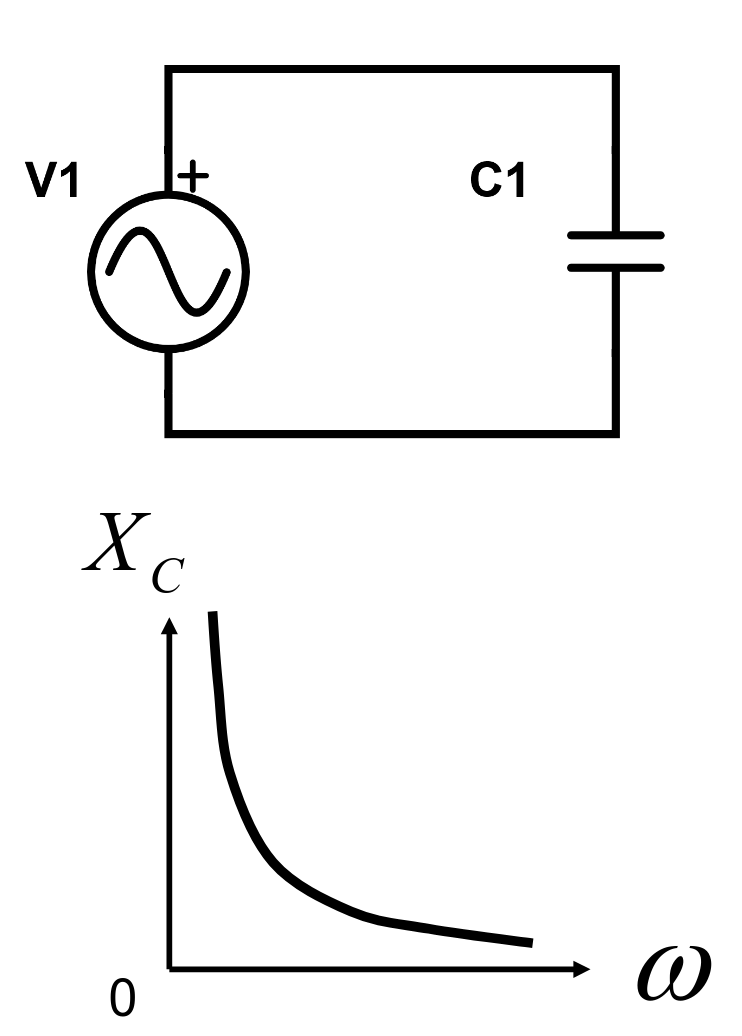
\includegraphics[width=.3\textwidth]{media/capacitive_reactance.png}
\end{center}

\efigbox{X_c = \dfrac{1}{\omega \cdot C}}
where:
\begin{itemize}
    \item $X_c$: capacitive reactance [Ohm];
    \item $\omega$: angular frequency [rad/s];
    \item $C$: capacitance [F = As/V].
\end{itemize}

\newpage
\subsection{Relationship between current and voltage on an ideal inductor}
\begin{center}
    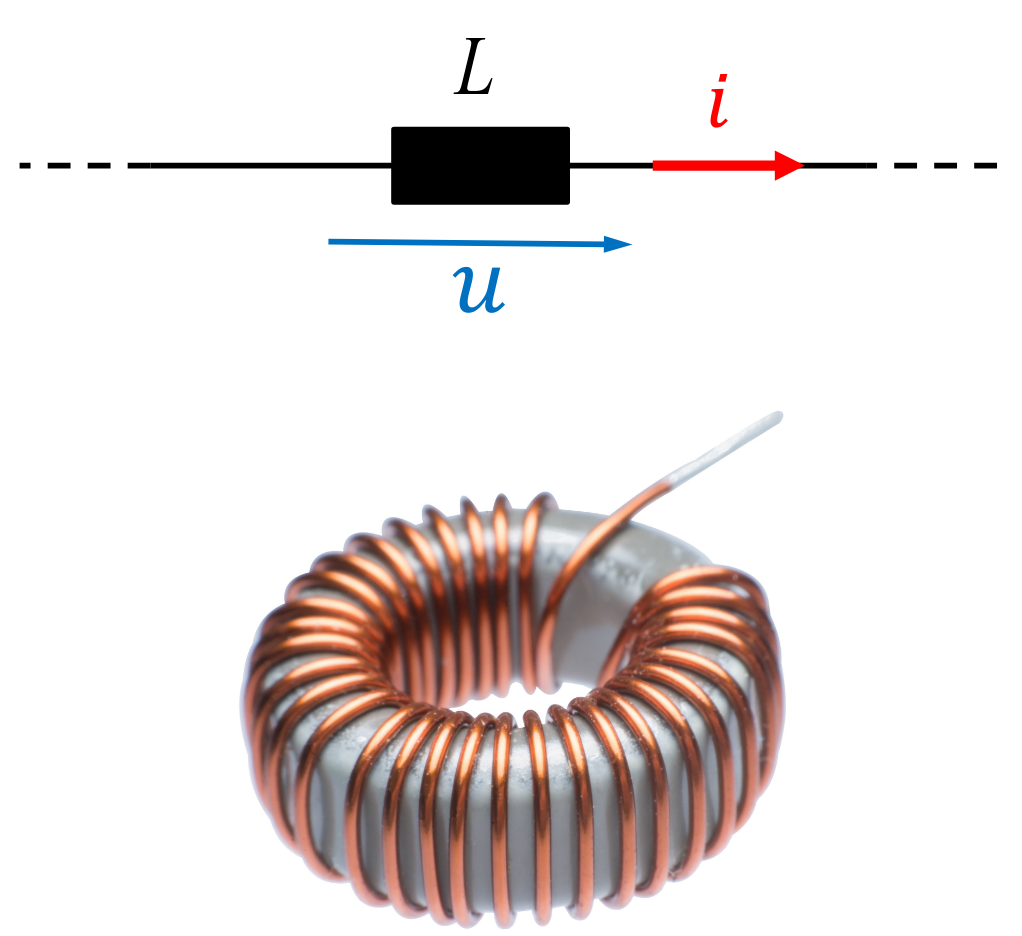
\includegraphics[width=.3\textwidth]{media/ideal_inductor.png}
\end{center}

\efigbox{u = L\cdot \dfrac{\Delta i}{\Delta t}}

\subsection{Inductive reactance $X_L$}
\begin{center}
    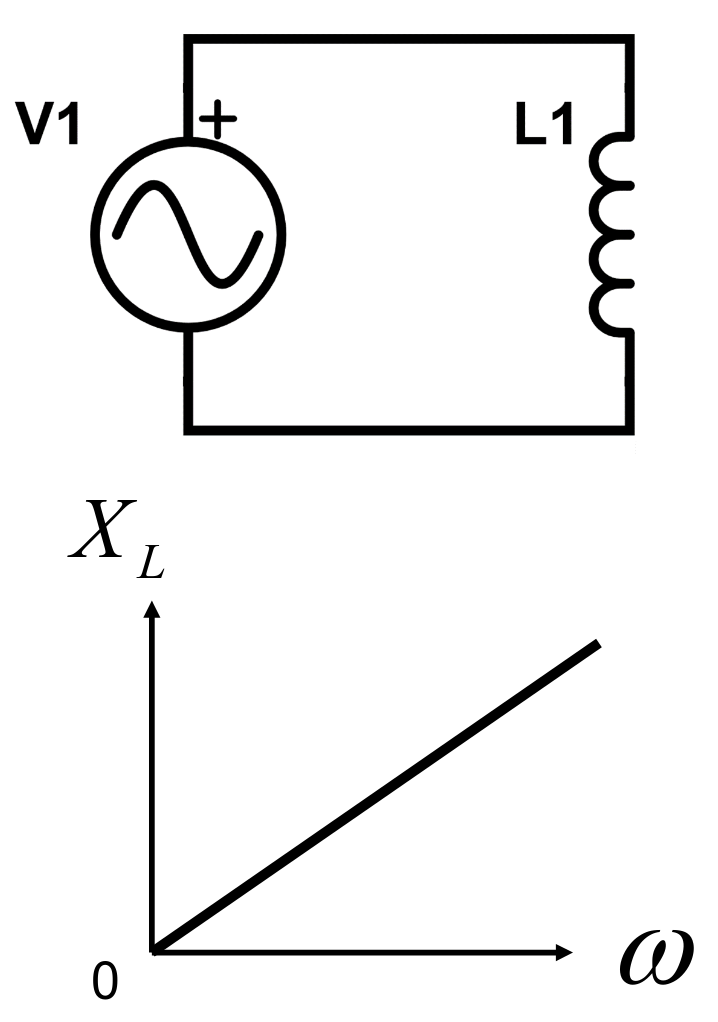
\includegraphics[width=.3\textwidth]{media/linear_capacitive_reactance.png}
\end{center}

\efigbox{X_L = \omega \cdot L}

where:
\begin{itemize}
    \item $X_L$: inductive reactance [Ohm];
    \item $L$: inductance [H];
    \item $\omega$: angular frequency [rad/s];
\end{itemize}

\newpage
\subsection{Vectors properties}
\subsubsection{Multiply}
The magnitude (es. the radius $r$ in polar representation) is
multiplied and the angle is added:
\efigbox{r_c = r_a\cdot r_b\\ \varphi_c = \varphi_a + \varphi_b}

\subsubsection{Divide}
The magnitude is devided and the angle is subtracted:
\efigbox{r_c = \dfrac{r_a}{r_b}\\ \varphi_c = \varphi_a - \varphi_b}

\subsection{Impedance $Z$}
The impedance is the ratio of voltage and current phasor. It's a complex number.

\efigbox{Z = \dfrac{u(t)}{i(t)}\\\\
        \left|Z\right| = \dfrac{\left|u(t)\right|}{\left|i(t)\right|}\\\\
        \angle Z = \angle u(t) - \angle i(t) = \Delta \varphi}

Therefore, the impedance corresponds to the AC resistance with phase shift:
\efigbox{\underline{Z} = \dfrac{\underline{U}}{\underline{I}} = \dfrac{U\angle \varphi_u}{I\angle \varphi_i} = Z\angle(\varphi_u - \varphi_i) = Z\angle\varphi_Z}

where:

\begin{minipage}{0.5\textwidth}
    \begin{itemize}
            \item $Z$: impedance [Ohm];
            \item $\underline{U}$: voltage phasor [V];
            \item $\underline{I}$: current phasor [A];
    \end{itemize}
\end{minipage}
\begin{minipage}{0.5\textwidth}
    \begin{itemize}
            \item $\varphi_u$: phase angle of the voltage [rad];
            \item $\varphi_i$: phase angle of the current [rad];
            \item $\varphi_Z$: phase angle of the impedance [rad].
    \end{itemize}
\end{minipage}

\subsubsection{Types of impendance}
The angle of the impedance $\varphi_Z$ indicates the type of impedance:
\begin{itemize}
    \item $\varphi_Z > 0^{\circ} \rightarrow$ voltage is ahead of current;
    \item $\varphi_Z = 0^{\circ} \rightarrow$ voltage and current are in phase;
    \item $\varphi_Z < 0^{\circ} \rightarrow$ current is ahead of voltage.
\end{itemize}

\vfill
\begin{center}
    \begin{tikzpicture}[line cap=round, line join=round, font=\bfseries]
        \fill[yellow!30] (0,0) rectangle (6,2);
        \fill[purple!30] (0,0) rectangle (6,-2);
    
        \draw[-Latex, thick, green!40!black] (0,0) -- (6,0) node[right] {pure ohmic};
        \draw[-Latex, thick, brown] (0,0) -- (0,2) node[above] {pure inductive};
        \draw[-Latex, thick, violet] (0,0) -- (0,-2) node[below] {pure capacitive};
    
        \node[anchor=west, black] at (0.15, 1) {inductive or ohmic-inductive};
        \node[anchor=west, black] at (0.15, -1) {capacitive or ohmic-capacitive};
    \end{tikzpicture}
\end{center}

\subsubsection{Graphical representation}
\begin{center}
    \begin{tikzpicture}[scale=1.5]
        % axis
        \draw[-Latex] (-2,0) -- (3,0) node[right] {$\mathrm{Re}\,(x)$};
        \draw[-Latex] (0,-2) -- (0,2.2) node[right] {$\mathrm{Im}\,(y)$};
        
        % circles
        \draw[red] (0,0) circle(1);
        \draw[blue] (0,0) circle(1.7);

        % vectors
        \draw[-Latex,very thick,blue] (0,0) -- (1.7,0) node at (1.3,-0.2) {$u(t)$};
        \draw[-Latex,very thick,red] (0,0) -- (0.8660254,0.5) node at (0.3,0.45) {$i(t)$};

        \draw[-Latex,thick] (0.8660254,0.5) -- (2.2,1.2701705922172) node at (1.8,1.25) {$Z$};
        \draw[-Latex,thick] (1.7,0) -- (2.2,0) node at (1.85,-0.2) {$R$};
        \draw[-Latex,thick] (2.2,0) -- (2.2,1.2701705922172) node[midway,right] {$X_L$};

        % angle
        \draw[Latex-Latex,thick,darkgreen] (1.225,0) arc (0:30:1.225) node at (1.4,0.35) {$\Delta\varphi$};
    \end{tikzpicture}
\end{center}

\subsection{Admittance $Y$}
The reciprocal of the impedance $Z$ is the admittance $Y$ and thus the ratio
of the current and voltage phasor. The admittance therefore corresponds to
the AC conductance with phase shift:

\efigbox{\underline{Y} = \dfrac{\underline{I}}{\underline{U}} = \dfrac{I\angle \varphi_i}{U\angle \varphi_u} = Z\angle(\varphi_i - \varphi_u) = Z\angle\varphi_Y\\\\
        \left|\underline{Y}\right| = \dfrac{1}{\left|\underline{Z}\right|}\Longrightarrow \varphi_Y = -\varphi_Z}

\subsection{Current and voltage relations}
\subsubsection{Resistor $R$}
\pph{Current-voltage relationship for instantaneous values}
\efigbox{u_R(t) = R\cdot i_R(t)}

\pph{Impedance = Ohmic resistance}
\efigbox{R=\frac{U_R}{I_R}\angle 0^{\circ}}

\begin{center}
    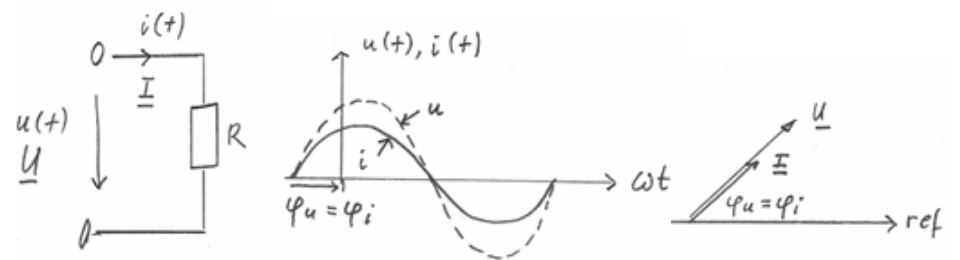
\includegraphics[width=.6\textwidth]{media/ohmic_resistance.png}
\end{center}

\subsubsection{Capacitor $C$}
\pph{Current-voltage relationship for instantaneous values}
\efigbox{i_C(t) = C\cdot \dfrac{du_C(t)}{dt}}

\pph{Impendance = Capacitive reactance}
\efigbox{X_C = \dfrac{U_C}{I_C} = \dfrac{1}{\omega\cdot C}\angle -90^{\circ}}

\begin{figure*}[ht!]
    \begin{center}
        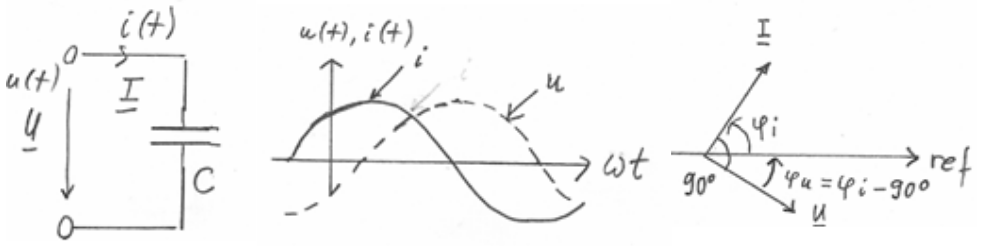
\includegraphics[width=.6\textwidth]{media/capacitive_reactance_Graph.png}
        \caption*{Current leads the voltage by 90 degrees}
    \end{center}
\end{figure*}

\subsubsection{Inductor $L$}
\pph{Current-voltage relationship for instantaneous values}
\efigbox{u(t) = L\cdot \dfrac{di(t)}{dt}}

\pph{Impendance = Inductive reactance}
\efigbox{X_L = \dfrac{U_L}{I_L} = \omega \cdot L\angle +90^{\circ}}

\begin{figure*}[ht!]
    \begin{center}
        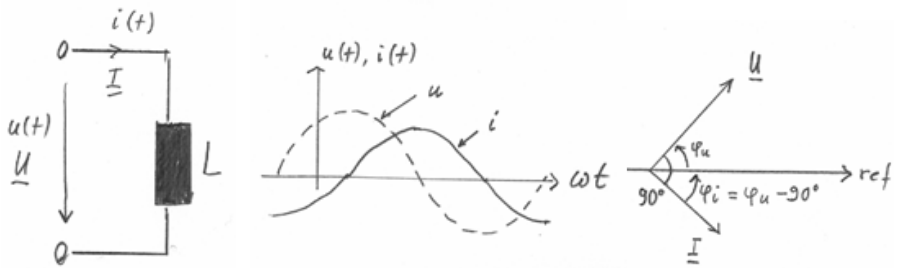
\includegraphics[width=.6\textwidth]{media/inductive_reactance.png}
        \caption*{Current lags the voltage by 90 degrees}
    \end{center}
\end{figure*}

\subsection{Impendance and admittance phasor with R, C and L}
\begin{center}
    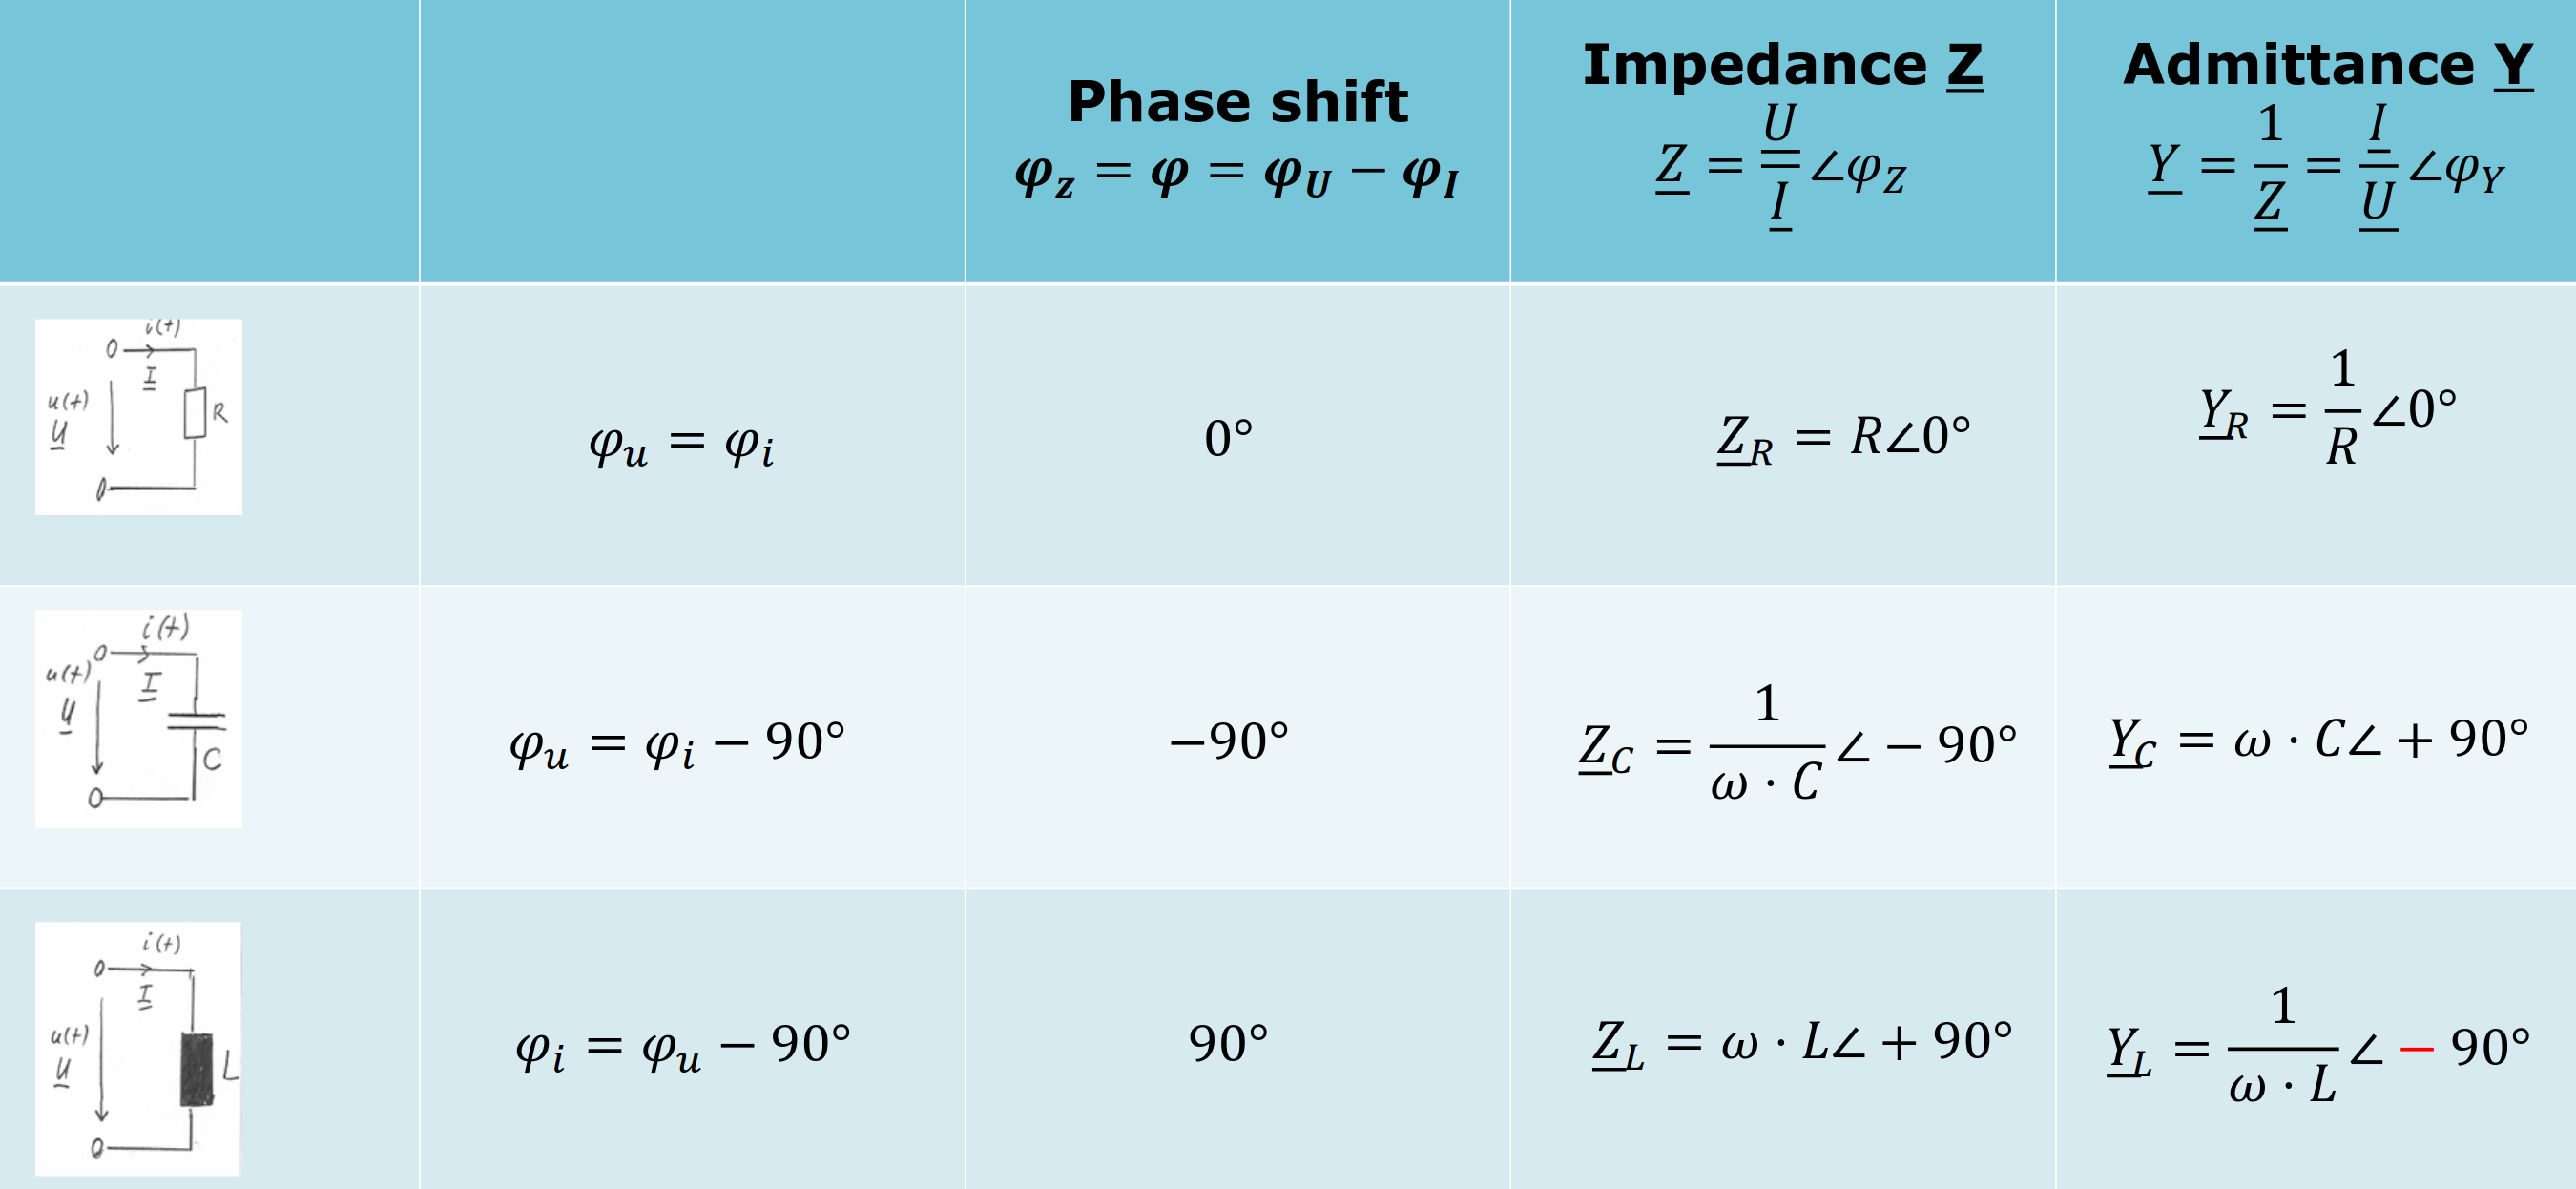
\includegraphics[width=\textwidth]{media/impedance_admittance.png}
\end{center}

\subsubsection{Series connection}
\pph{Resistances}
\begin{center}
    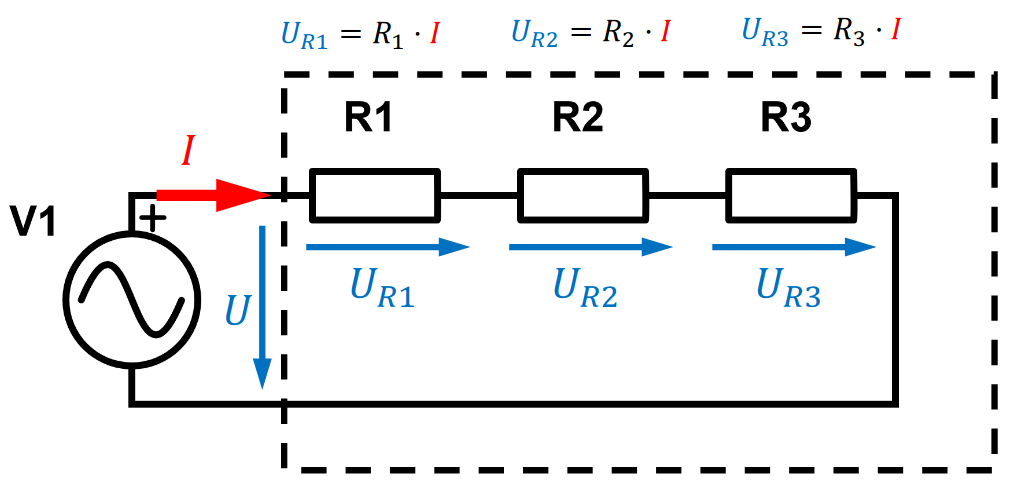
\includegraphics[width=.5\textwidth]{media/series_resistances.png}
\end{center}

\efigbox{R_{\text{equi}} = \dfrac{U}{I} = \dfrac{U_{R1}+U_{R2}+U_{R3}}{I} = R_1 + R_2 + R_3}

\pph{Impedances}
\begin{center}
    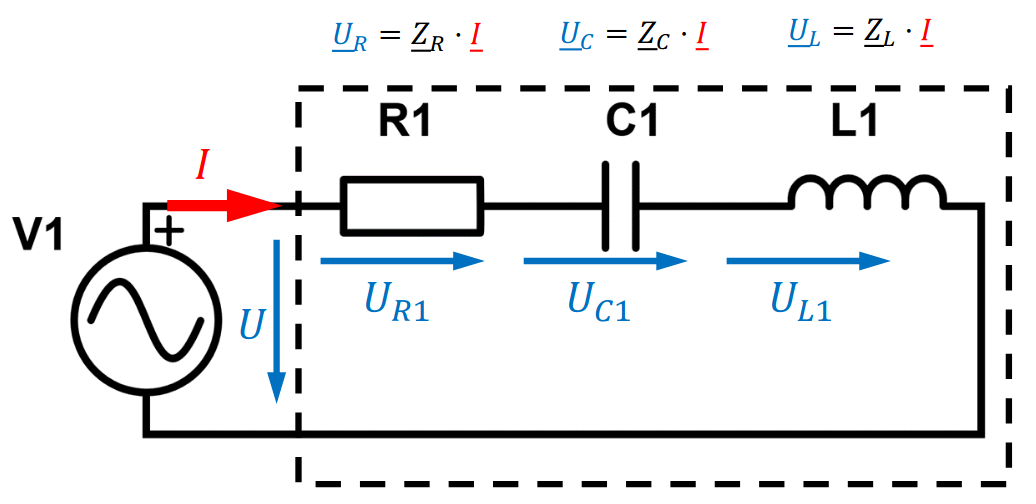
\includegraphics[width=.5\textwidth]{media/series_impedances.png}
\end{center}

\efigbox{Z_{\text{equi}} = \dfrac{\underline{U}}{\underline{I}} = \dfrac{U_{R1}\angle0^{\circ} + U_{C1}\angle-90^{\circ} + U_{L1}\angle+90^{\circ}}{I\angle0^{\circ}} = \underline{Z_1} + \underline{Z_2} + \underline{Z_3}}

\newpage
Adding voltages in series connection means adding impedances:

$\underline{U_R} = \underline{Z_R} \cdot \underline{I} = R\cdot\angle\varphi_i\\\\
\underline{U_L} = \underline{Z_L} \cdot \underline{I} = X_L\angle 90^{\circ} \cdot\angle\varphi_i\\\\
\underline{U_C} = \underline{Z_C} \cdot \underline{I} = X_C\angle -90^{\circ} \cdot\angle\varphi_i$

\begin{center}
    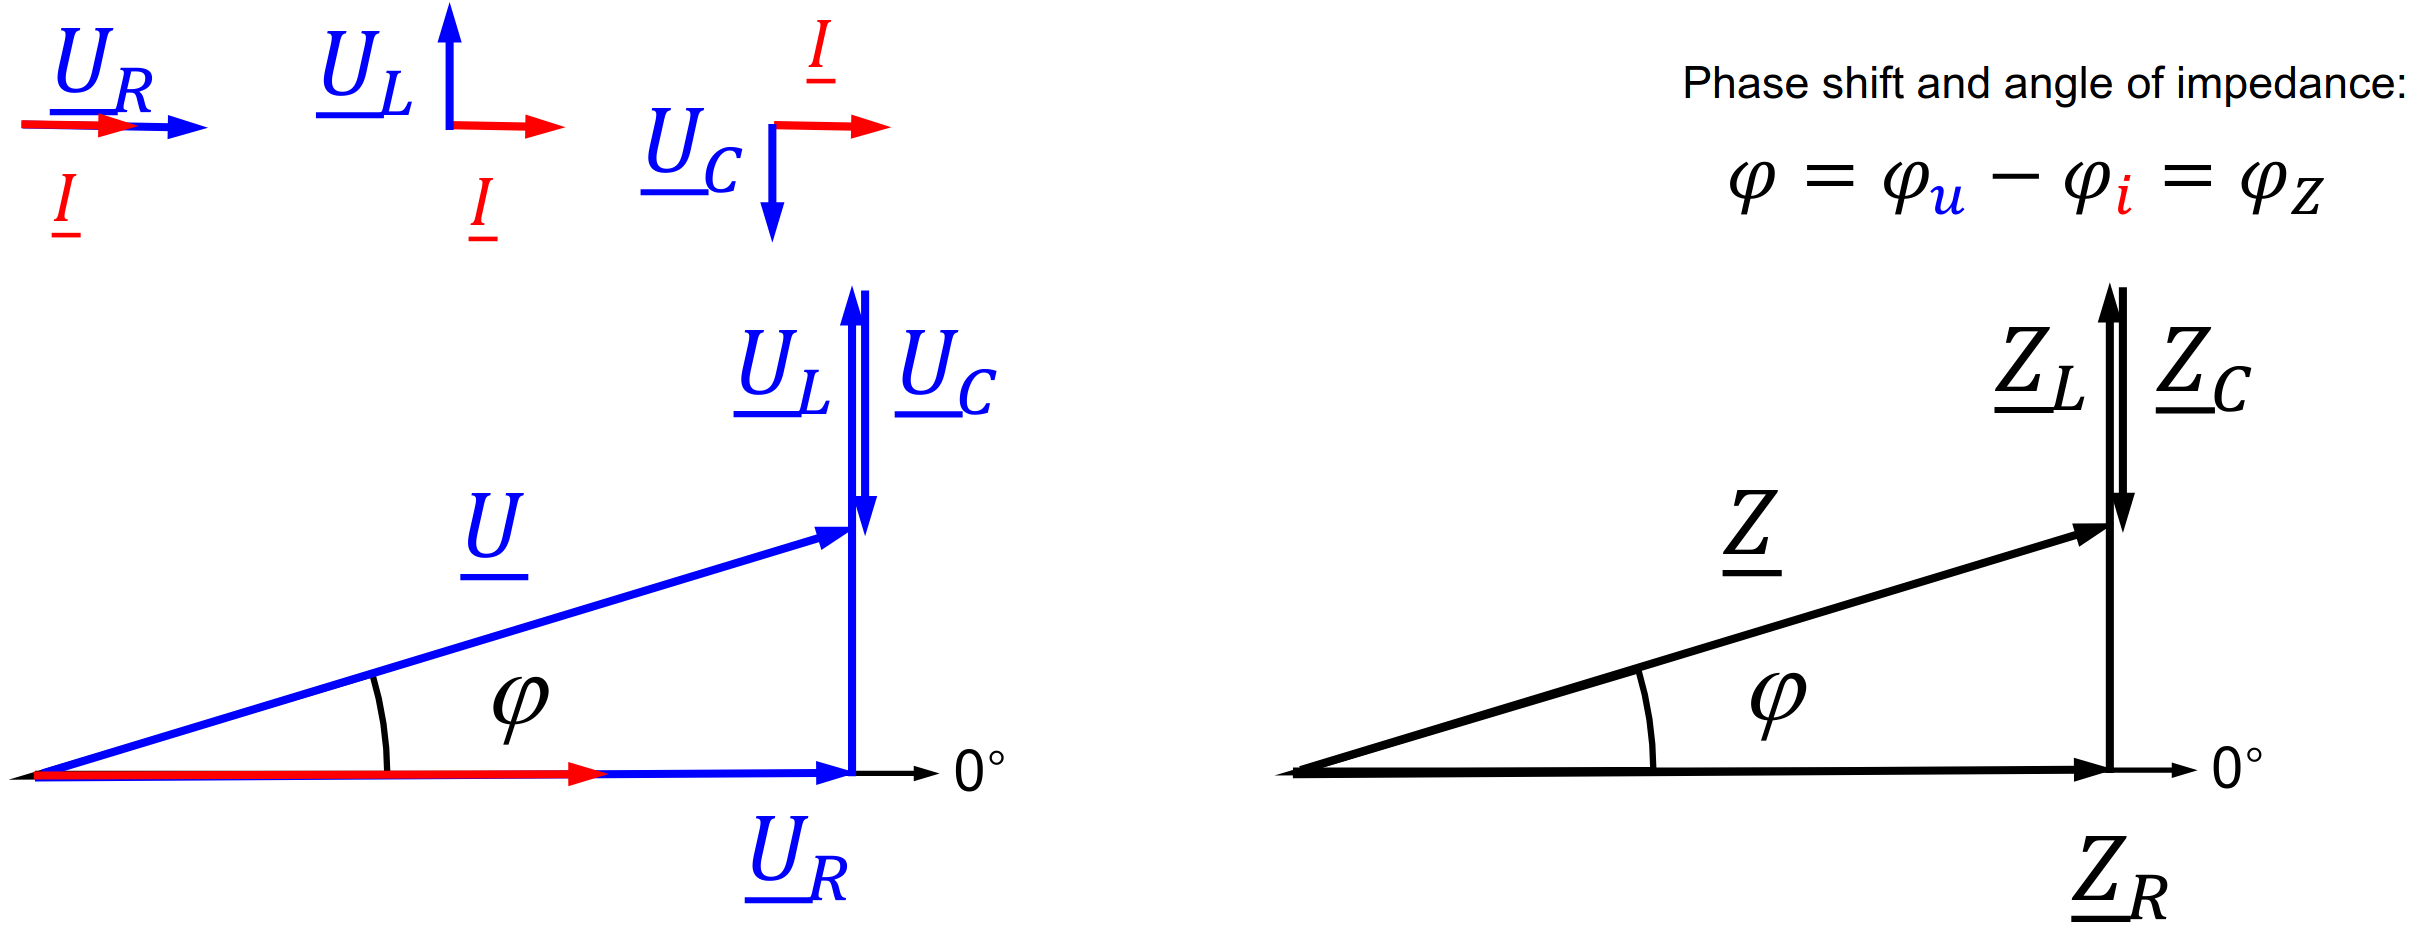
\includegraphics[width=.8\textwidth]{media/voltage_impedance.png}
\end{center}

\efigbox{Z_{\text{eq}} = Z_1 + Z_2 + Z_3}

\subsubsection{Parallel connection}
\pph{Resistances}
\begin{center}
    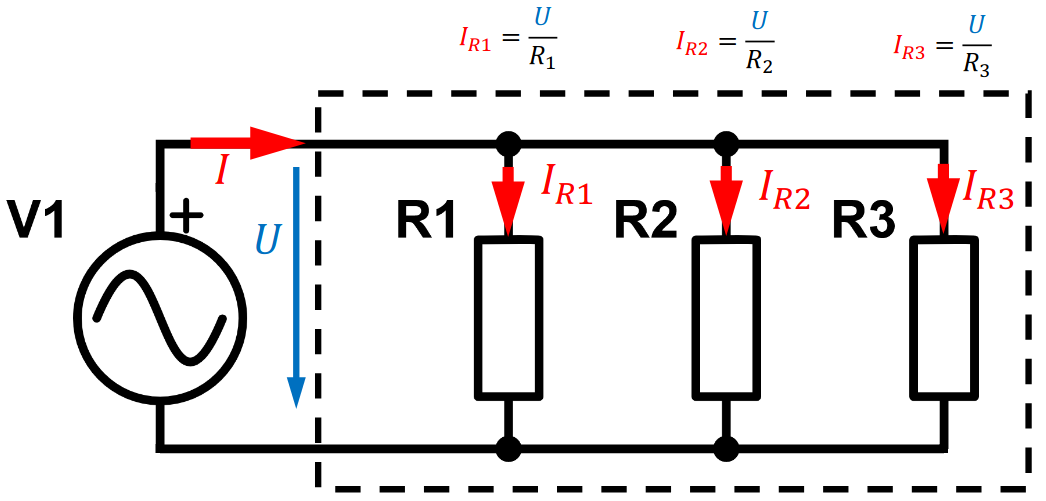
\includegraphics[width=.5\textwidth]{media/parallel_resistances.png}
\end{center}
\efigbox{R_{text{equi}} = \dfrac{U}{I} = \dfrac{1}{\frac{1}{R_1} + \frac{1}{R_2} + \frac{1}{R_3}} = \dfrac{1}{G_1 + G_2 + G_3}}

\pph{Impedances}
\begin{center}
    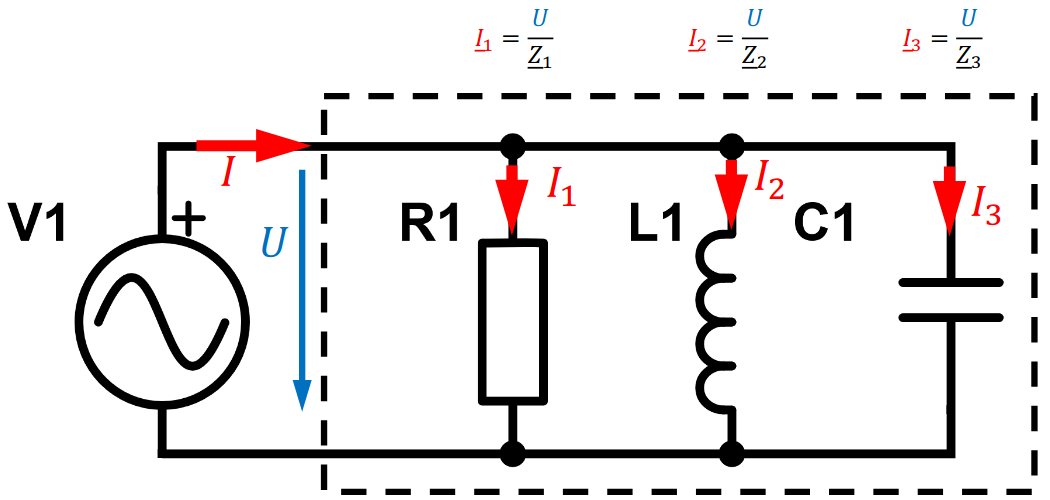
\includegraphics[width=.5\textwidth]{media/parallel_impedances.png}
\end{center}
\efigbox{Z_{\text{equi}} = \dfrac{\underline{U}}{\underline{I}} = \dfrac{U}{I\angle0^{\circ}} = \dfrac{1}{\dfrac{1}{\underline{Z_1}} + \dfrac{1}{\underline{Z_2}} + \dfrac{1}{\underline{Z_3}}} = \dfrac{1}{\underline{Y_1} + \underline{Y_2} + \underline{Y_3}}}

\newpage
Adding currents in parallel connection means adding admittances:

$\underline{I_R} = \dfrac{\underline{U_R}}{\underline{Z_R}} = \dfrac{U}{R}\cdot\angle\varphi_u\\\\\\
\underline{I_L} = \dfrac{\underline{U_L}}{\underline{Z_L}} = \dfrac{U}{X_L}\angle\varphi_u -90^{\circ}\\\\\\
\underline{I_C} = \dfrac{\underline{U_C}}{\underline{Z_C}} = \dfrac{U}{X_C}\angle\varphi_u +90^{\circ}$
\begin{center}
    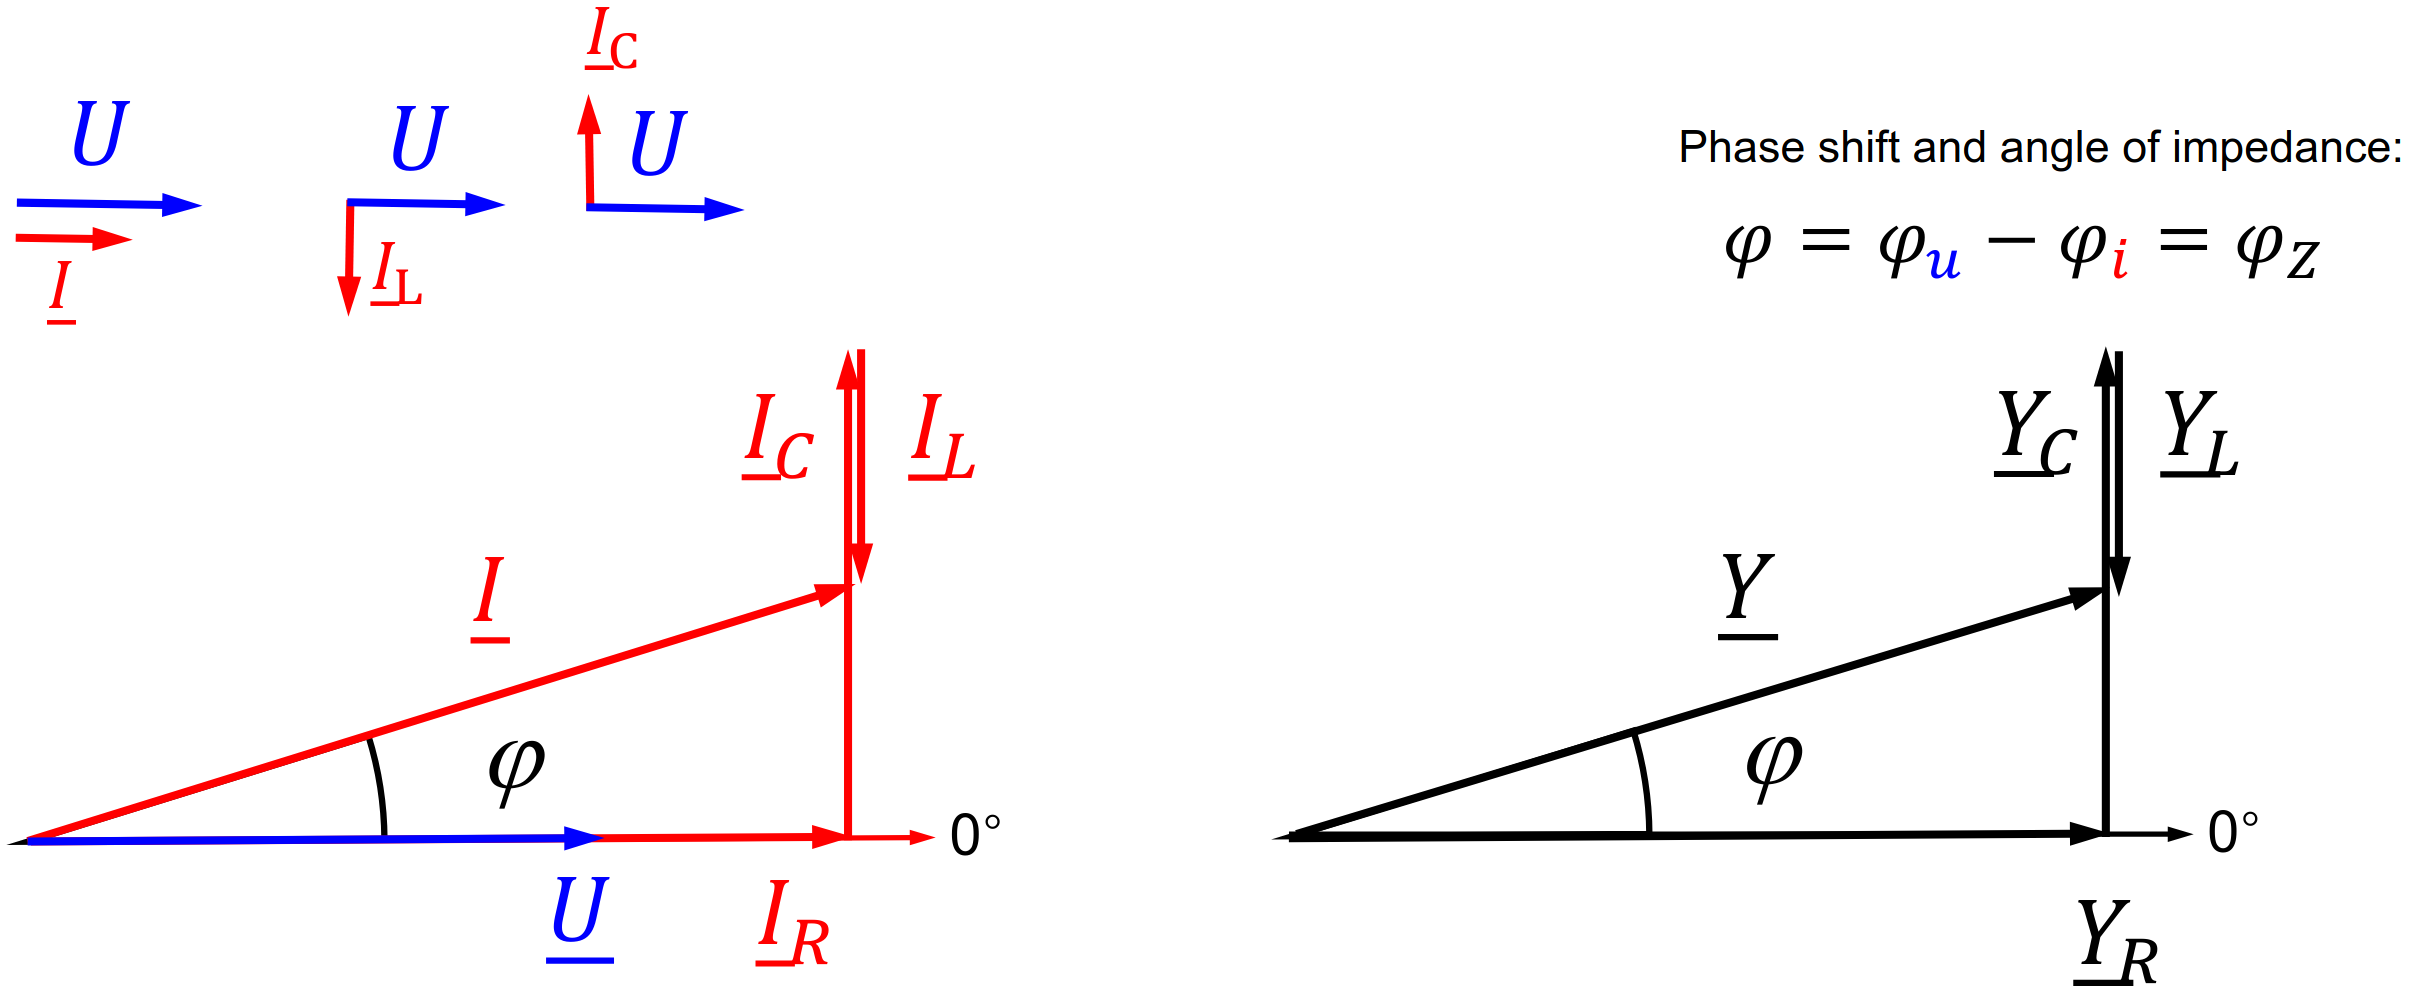
\includegraphics[width=.8\textwidth]{media/current_admittance.png}
\end{center}
\efigbox{\underline{Z_{\text{eq}}} = \dfrac{1}{\underline{Y_1} + \underline{Y_2} + \underline{Y_3}}}

\subsection{AC newtwork analysis}
AC network analysis is similar to DC network analysis but calculated with phasors.

\subsubsection{Kirchhoff's current law (KCL)}
\efigbox{\underline{I_1} + \underline{I_2} + ... + \underline{I_n} = \dsum{k=1}{n} \underline{I_k} = 0}

\subsubsection{Kirchhoff's voltage law (KVL)}
\efigbox{\underline{U_1} + \underline{U_2} + ... + \underline{U_n} = \dsum{k=1}{n} \underline{U_k} = 0}

\subsubsection{Voltage and current phasor relationship for circuit elements}
\efigbox{\underline{U} = \underline{Z}_{\text{Element-type}} \cdot \underline{I}}













\end{document}
